\documentclass[11pt]{article}
\usepackage[utf8]{inputenc}
\usepackage{graphicx}
\usepackage[english]{babel}
\usepackage{url}
\usepackage{float}
\usepackage[backend=bibtex,style=alphabetic,sorting=ynt]{biblatex}
\usepackage[dvipsnames]{xcolor}
\usepackage[left=3cm, right=3cm, top=2.5cm, bottom=2cm]{geometry}
\addbibresource{literatur.bib}
\graphicspath{ {./images/} }
\title{
{Construction and Validation of a Guideline for migrating a Microservice Architecture to Function as a Service}\\
{\large Frankfurt University of Applied Sciences}\\}
\author{Gianni Pasqual}
\date{18.03.2020}
\begin{document}
\maketitle
\newpage
{\Large \textbf {Abstract}}
\\\\ 
Mit der Technologie Function as a Service ist nach der Microservice-Architektur eine noch feinere Modularisierungsstufe von Software erreicht worden. Mit dieser ist es möglich Software noch schneller bereitzustellen und im gleichen Zuge Einsparungen bei dem Betrieb der IT-Infrastruktur zu erzeielen. Dies erscheint auf den ersten Blick natürlich sehr lokrativ für viele Unternehmen, jedoch sollte die Entscheidung für den teilweisen oder gesamten Umzug der Service-Landschaft wohl überlegt sein. Wie bei jeder anderen Technologie hat auch diese ihre Potentiale und Herausforderungen die gemeistert werden müssen. Für Unternehemn, die sich dazu entschieden haben Function as a Service (FaaS) in ihre Infrastruktur einzubinden, soll diese Arbeit als Orientierung bei der Migration dienen. Da viele Unternehmen bereits von den monolithischen Anwendungen auf kleinere modularere Services umgestiegen sind, geht diese Arbeit von einer bereits vorliegenden Microservice-Architektur aus. Es gilt herauszufinden in welchem Maße und ob überhaupt strukturelle Anpassungen vorgenommen werden müssen, als auch der Frage nach "Best-Practices", nach nun knapp vier Jahren des Bestehens, nachzugehen.
\\\\ 
Zudem soll sich vor allem mit dem von den verschiedenen Anbietern ausgehenden Vendor-Lock-In auseinadner gesetzt werden und erarbeitet werden, welche Möglichkeiten bestehen, diesen zu umgehen bzw. zu mildern. Um mögliche Schwächen des Leitfadens aufzuzeigen, soll dieser beispielhaft an einem Service erprobt werden und auftretenden Fehler dokumentiert und behandelt werden.
\newpage
{\Large \textbf {Index of abbreviations}}
\\\\ \\
\begin{tabular}{ p{2cm} p{10cm}} 
ADF & Azure Durable Functions \\
API & Application Programming Interface \\
ASF & Amazon Step Functions \\
AWS & Amazon Web Services \\
BaaS & Backend as a Service \\
BDD & Behaviour Driven Development \\
BFF & Backends for Frontends \\
CaaS & Container as a Service \\  
CD & Continuous Delivery \\  
CI & Continuous Integration \\
CLI & Command Line Interface \\
CNCF & Cloud Native Computing Foundatino \\
CPU & Central Processing Unit \\
CRD & Custom Resource Definition \\
DevOps & Development and Operations \\  
DEV & Development \\
DSL & Domain Specific Language \\
FaaS & Function as a Service \\ 
HPA & Horizontal Pod Autoscaler \\
IAM & Identity Access Management \\
IaaS & Infrastructure as a Service \\
IaC & Infrastructure as Code \\
INT & Integration (Testing) \\
IT & Information Technology \\
JVM & Java Virtual Machine \\
NIST & National Institute of Standards and Technology \\
OOP & Object Oriented Progamming \\
OS & Operating System \\
PaaS & Platform as a Service \\
POM & Project Object Model \\
PR & Pull Request \\
PRD & Production (Environment) \\
RPC & Remote Procedure Call \\
SAM & Serverless Application Model \\
SDK & Software Development Kit \\
UAT & User-Acceptance (Testing) \\
VCS & Version Controle System \\
XaaS & Anything as a Service \\
\end{tabular}
\newpage
\tableofcontents
\newpage
\section{Introduction}
\subsection{Objectives and Goals}
\subsection{Problem Statement}
\subsection{Thesis Structure}










\section{Background}
Ist eine Technologie, wie Function as a Service, noch relativ jung, so sind die Schritte der Findung einer in sich schlüssigen und allgemein vertretenen Definition oftmals noch nicht abgeschlossen. Auch bei der Definition von FaaS, Serverless und der Einordung dieser beiden Konzepte in die Infrastruktur des Cloud Computings8  \cite{mell2011nist}, ist dieser Prozess noch im Gange, wobei mitlerweile die unterschiedlichen Definitionen der offentlichen FaaS- und Serverless-Anbieter einige Gemeinsamkeiten aufweisen. Trotz alledem bestehen weiterhin Ungenauigkeiten, die es in den nächsten Jahren noch zu beseitigen gilt. Hierzu später mehr.\\\\ 


\subsection{Definition Cloud Computing}
Regarding a technology report, the term cloud computing can be traced back to the year 1996, where it initially has been used in a business plan from the company Compaq \cite{regalado2011coined}. According to Regalado, several developers used the term cloud computing to discuss the future of internet business. \\\\
The basic concept of cloud computing is its dynamic, scalable, reliable and unlimited provisioning of resources via the internet. Over time, its concept has raised attention in literature but never became popular until 2006 \cite{fox2009above}. In 2006 AWS released Elastic Compute Cloud (EC2), followed by Google with its App Engine in 2008. With those two products, the interest in cloud computing started to launch, and other companies like Heroku started to provide PaaS services as well. Even in that early state, Google introduces a stateful and a stateless layer into App Engine. The stateful layer was used to store and keep track of the actual state of the application, and the stateless layer was used to execute the applications inherent business logic \cite{fox2009above}. In 2009 Berkeley released a study on the six most promising potentials of cloud computing that have been implemented by today different XaaS-Concepts, which are listed in the following: \\ 
\begin{itemize}
\item[1.] The appearance of infinite computing resources on demand. 
\item[2.] The elimination of an up-front commitment by cloud users.
\item[3.] The ability to pay for use of computing resources on a short-term basis as needed.
\item[4.] Economies of scale that significantly reduced cost due to many, very large data centers.
\item[5.] Simplifying operation and increasing utilization via resource virtualization.
\item[6.] Higher hardware utilization by multiplexing workloads from different organizations.
\end{itemize}
After 16 previous definitions, the National Institute of Standards and Technology (NIST) published a final definition on cloud computing in 2011, that is referred to in several papers \cite{mell2011nist}. The definition, according to NIST, describes cloud computing as a model consisting of five essential characteristics, three service models - IaaS, PaaS and SaaS, respectively - as well as four deployment models. \\\\\textit{"Cloud Computing is a model for enabling ubiquitous, convenient, on-demand network access to a shared pool of configurable computing resources (i.e., networks, servers, storage, applications, and services) that can be rapidly provisioned and released with minimal management effort or service provider interaction. "} \cite{mell2011nist}. \\\\Roughly speaking, the five essential characteristics are, the ability to automatically provision resources based on present demands (\textit{on-demand self-service}), the ability to access them from all common devices (\textit{broad network access}), the ability to distribute resources as efficient as possible to those consumers which currently need them, whereas the exact physical position of these resources do not matter to the consumer (\textit{resource pooling}), the ability to automatically scale resources, based on incoming traffic (\textit{rapid elasticity}) and the possibility to monitor and limit resource utilization, which has to be transparent to the customer (\textit{measured service}). \\\\With the service models, only IaaS, PaaS and SaaS are distinguished. Other XaaS-solutions like FaaS and BaaS have not been invented at that time, but they do follow the described pattern. According to NIST, four different deployment models exist, that can be used to provide the application code to the cloud provider. Using a \textit{private cloud} approach, it is the companies responsibility to provision its infrastructure. The infrastructure itself does not necessarily need to be hosted on-premise and can be obtained from a third party PaaS or IaaS provider. With the deployment to a \textit{community cloud}, several companies share the same cloud, that is either operated jointly by them or provided by a third party. Second, to the last, there is the possibility to use the \textit{public cloud}, in which the company uses the facilities and resources of a third-party provider. The last deployment model is the so-called \textit{hybird cloud} approach, which is a combination of several aspects from the previous three \cite{mell2011nist}.
\begin{figure}[H]
\caption{Overview of Cloud Computing Service-Models}
\label{fig:cloudComputingConcepts}
\centering
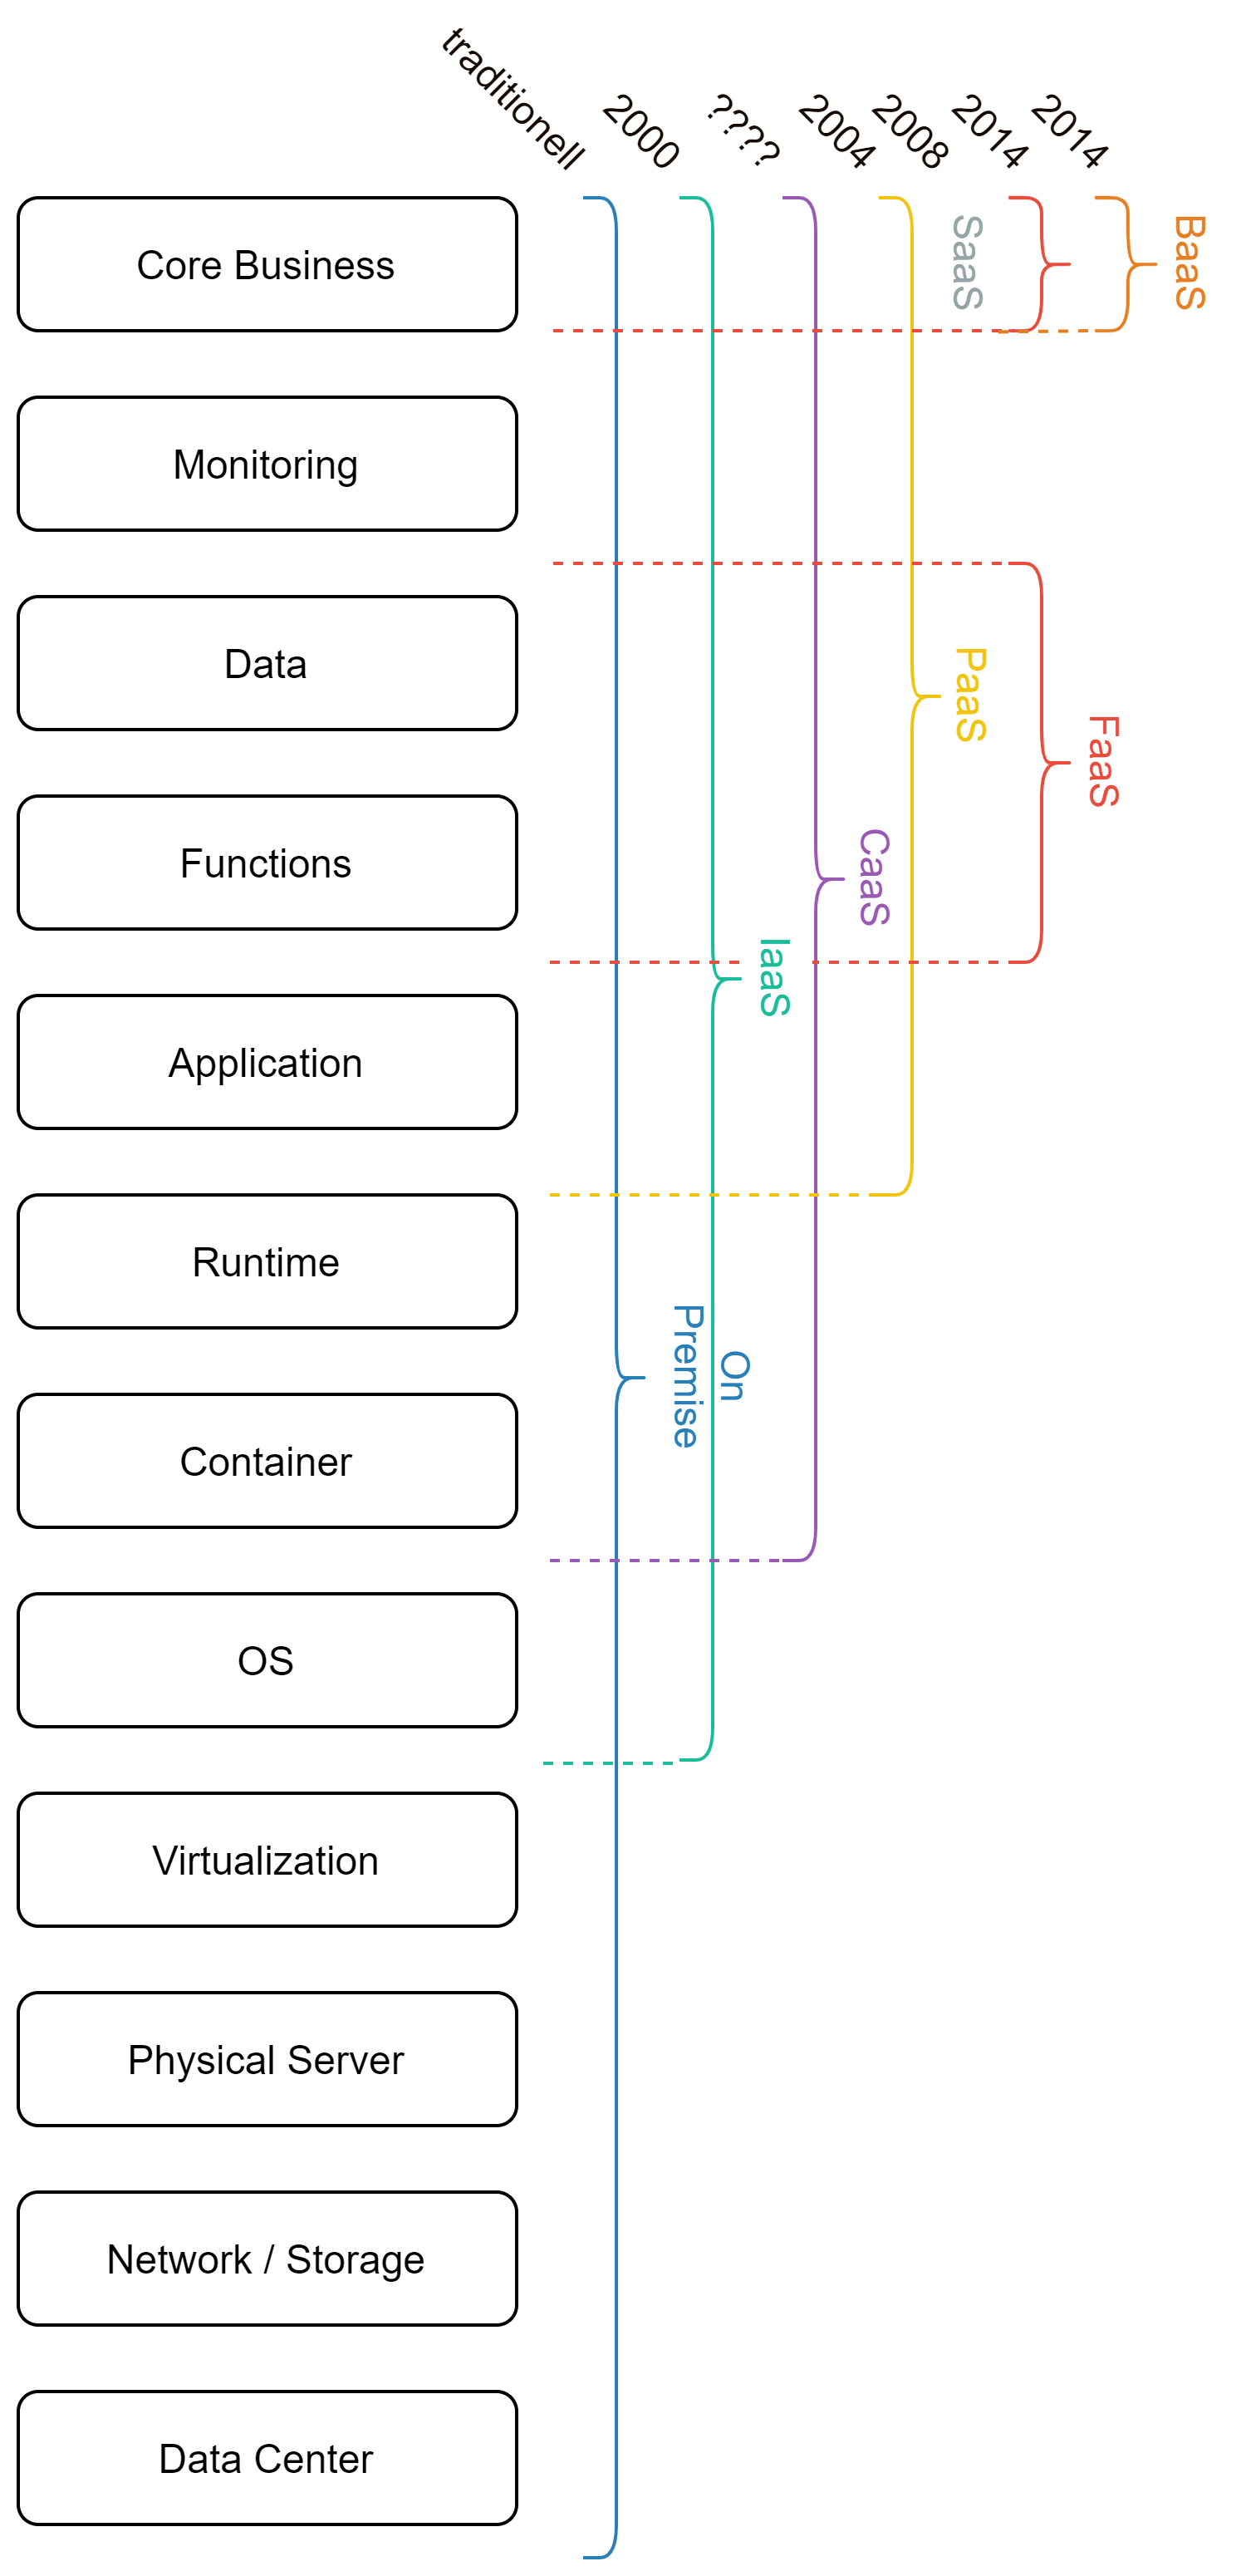
\includegraphics[angle=90,width=1\textwidth]{serviceModels}
\end{figure}
Besides the three mentioned cloud computing models depicted by NIST, and the marked BaaS and FaaS solutions, others exist as well, that are depicted in figure ~\ref{fig:cloudComputingConcepts}. The displayed cloud concepts have evolved over time from 2011 until today. Figure ~\ref{fig:cloudComputingConcepts} provides a gross overview of their level of operation and the year they have been introduced. 


\subsection{Function as a Service}
Function as a Service is a so-called \textit{serverless} cloud computing concept, which initially was introduced by AWS Lambda in 2014. In 2014 Lambda was only available as a preview release and launched for commercial usage in 2015 \footnote{https://docs.aws.amazon.com/lambda/latest/dg/lambda-releases.html}. Almost one year later, Microsoft, Google and IBM entered the market as well, with Azure Functions, Google Cloud Functions and OpenWhisk, respectively. Regarding IaaS and PaaS, Function as a Service further abstracts operational tasks, such as provisioning of resources, monitoring, scaling, failure recovery and availability, away from the developer toward the platform. The market around Function as a Service has evolved steadily and meanwhile offers a vast number of open-source and proprietary cloud providers. A detailed overview of the existing solutions is provided by the CNCF\footnote{https://github.com/cncf/wg-serverless}. Moreover, CNCF provides an overview of tools, which is dealt with in a later section.\\\\ 
Due to FaaS being a relatively new technology, there is no official documentation or reference architecture as i.e. provided for Cloud Computing by NIST. The consequence is a lack of the underlying architecture and different implementation of the providers, resulting in inconsistency. The lack of uniform implementation over the existing platforms exacerbates multi-cloud solutions across them \cite{mell2011nist}.
Nonetheless, there is consensus on the definition and functionality of FaaS across the providers, for the most part. Microsoft i.e. defines Azure Azure Functions as an \glqq \textit{[...] event-driven serverless compute platform that can also solve complex orchestration problems. Build and debug locally without additional setup, deploy and operate at scale in the cloud, and integrate services using triggers and bindings.} \grqq{}\footnote{https://azure.microsoft.com/en-us/services/functions/}. With that definition, Microsoft does not describe the operational benefits of FaaS but its technical capabilities. The concept should be used to define certain events that are activated by the occurrence of predefied trigger, which could be a HTTP-call, and bindings to a database or another service. Looking at the definition of AWS Lambda, the same technical benefits are described: \glqq \textit{AWS Lambda [...] runs your code in response to events [,] automatically manages the underlying compute resources [...] [and] extend[s] other AWS services with custom logic [...]}\grqq{} but also the operational benefits are taken into account \glqq \textit{[...][Lambda] performs all the administration of the compute resources, including server and operating system maintenance, capacity provisioning and automatic scaling, code and security patch deployment, and code monitoring and logging. All you need to do is supply the code.}\grqq{}\footnote{https://aws.amazon.com/lambda/}.\\\\
Besides the basic event-based HTTP-triggers and scheduled Function invocations, most solutions, both open-source and proprietary, provide one more trigger that strongly depends on the underlying platform. This trigger, as mentioned by Microsoft, is the binding to other services supplied by the platform. Events of a function are connected to the different BaaS solutions of the platform, further discussed in\textit{Dissociation of FaaS and Serverless}. They are triggered when something in a database changes, a new user was registered or a Push-Notification -like AWS SSN or Google Pub/Sub etc\.- needs to be sent.\\
\begin{figure}[H]
\caption[FaaS Programming Model nach OpenWhisk]{\footnote{http://OpenWhisk.apache.org/documentation.html}}
\label{fig:OpenWhiskProgrammingModel}
\centering
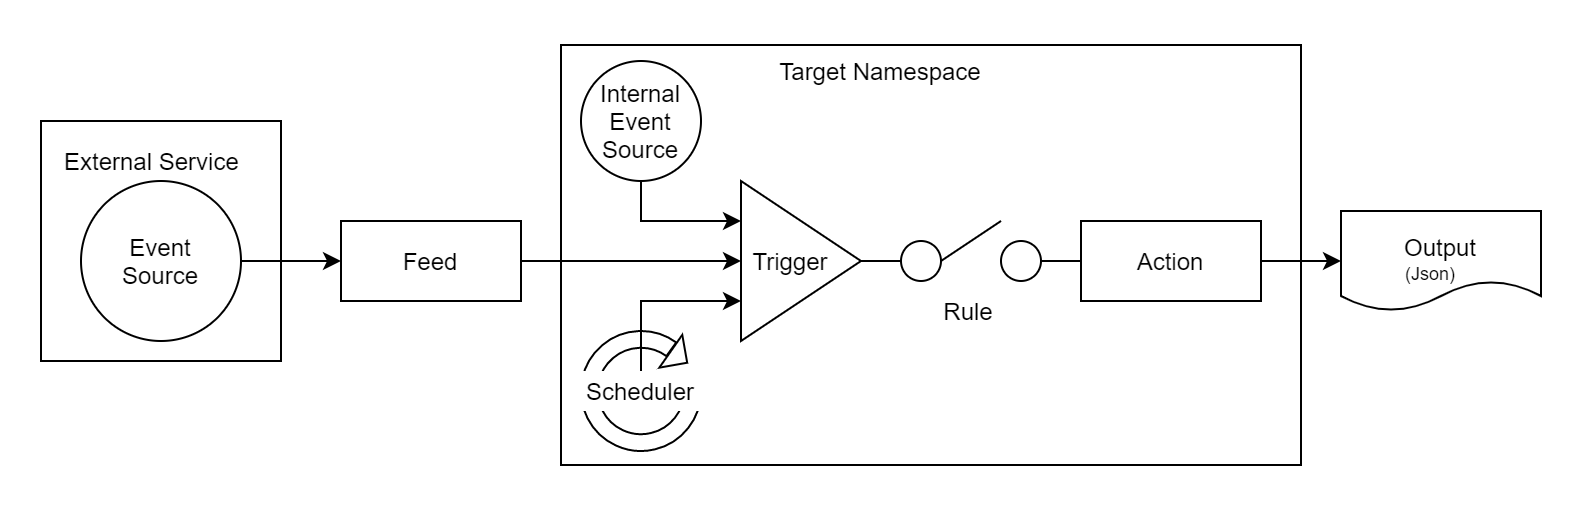
\includegraphics[width=1\textwidth]{ProgrammingModel}
\end{figure}
Figure ~\ref{fig:OpenWhiskProgrammingModel}, based on OpenWhisk, provides an overview of the different types of event-triggers that are currently used by the three largest FaaS-providers, namely AWS, Azure and OpenWhisk. Due to OpenWhisk, formerly being backed by a large company (IBM), in literature, its model is often used as a reference for the other FaaS implementations of the other cloud vendors. It can be assumed that the architectural concept of FaaS at the other providers is not that different from OpenWhisk, because it is supplied in a large cloud environment (IBM) \cite{van2019spec}. Currently, OpenWhisk is developed as an open-source framework, backed by Apache. \\ Another fundamental concept of FaaS, which is in accordance with the fifth essential characteristic of the NIST definition on cloud computing, the \textit{measured service}, is its scalability by the so-called pay-per-use model. It ensures that the customer only pays for the resources and computing capacity he used and not for the ones reserved, i.e. to cope with possible increases in traffic.\\ What can not be seen on the picture, but is essential to FaaS, is its statelessness, as further discussed in \textit{Benefits and Drawbacks}. Even though the container the functions runs in do have an application state inherent to them, utilizing that state is not an option. Functions are only active for a certain period and automatically will be discarded when reaching the limit of the platform. Therefore a request hitting a \textit{warm} function technically can access its state and do a calculation on it, but it is uncertain by which container an incoming request is served. \\\\
%\textcolor{blue}{Grundsätzlich ist zwar der Preis der für das Laufen einer einminütigen Funktionsaussführung verglichen mit dem Laufen des selben Codes auf einem von den Ressourcen her ähnlich bestückten PaaS-Server günstiger \cite{jonas2019cloud}, jedoch der Anwendungszweck ein ganz anderer. Während mit PaaS Anwendungen bedient werden, die eine dauerhaft hohe Nachfrage erfahren, sollen mit Funktionen primär einfache stark frequentierende Aufgaben geläst werden, bei denen der Nutzer nur für die Ressroucen bezahlen muss die die Funktion bei dem Aufruf nutzt und nicht für jene die ohen einkommende Aufrufe provisioniert wurden.}\\\\
Another important point, which can be found with other providers as well, is registered in the definition of OpenWhisk. On the one hand developers \glqq \textit{[...] can focus on building amazing and efficient applications [...]}\grqq{}, the other hand \glqq \textit{[...] developers [are writing] functional logic [...] in any supported programming language, that can be dynamically scheduled [...]}\grqq{}\footnote{http://OpenWhisk.apache.org/}. The former account the abstraction of servers, infrastructure and maintenance, at least to some extent. For the developer, it is not necessary to have any knowledge about the functioning of the underlying OS or the like, to provide working code snippets or an entire application. To be put in exaggeration, the developer cannot even configure the platform, whereas the only thing left, is to rely on the code he writes. By abstracting most of the provisioning tasks to the platform, the developer can only control aspects the provider allows him to control. The latter aims on a variety of programming languages. This is not solely a benefit of Function as a Service and also applies to other architectures like microservices.
Nevertheless, it provides the developer with more flexibility addressing a wider group of potential users.\\\\
%\textcolor{red}{Of course, these properties are connected with inevitable vendor lock-in, but this is neither bad nor good and should instead be soberly analyzed on its benefits and drawbacks. connected, since this makes decisions about the infrastructure, more about}\\\\
Figure ~\ref{fig:FaaSBaaSExample} depicts the general functioning of Function as a Service in a broader context. On the top right, the function-pool can be seen. When the developer uploads functions to the platform for later execution, the function will be stored in the function pool until it gets triggered. As soon as a trigger activates the function, a copy of the function will be instantiated. Before the actual business logic of the function can be processed, necessary modules and libraries, as well as other dependencies, need to be loaded. Depending on the frequency a function is triggered by clients, the process of instantiating new function copies, based on the function in the function-pool, will be repeated.    
\begin{figure}[H]
\caption{Anwendung mit FaaS und (P)BaaS, angelehnt an \cite{shafiei2020serverless}}
\label{fig:FaaSBaaSExample}
\centering
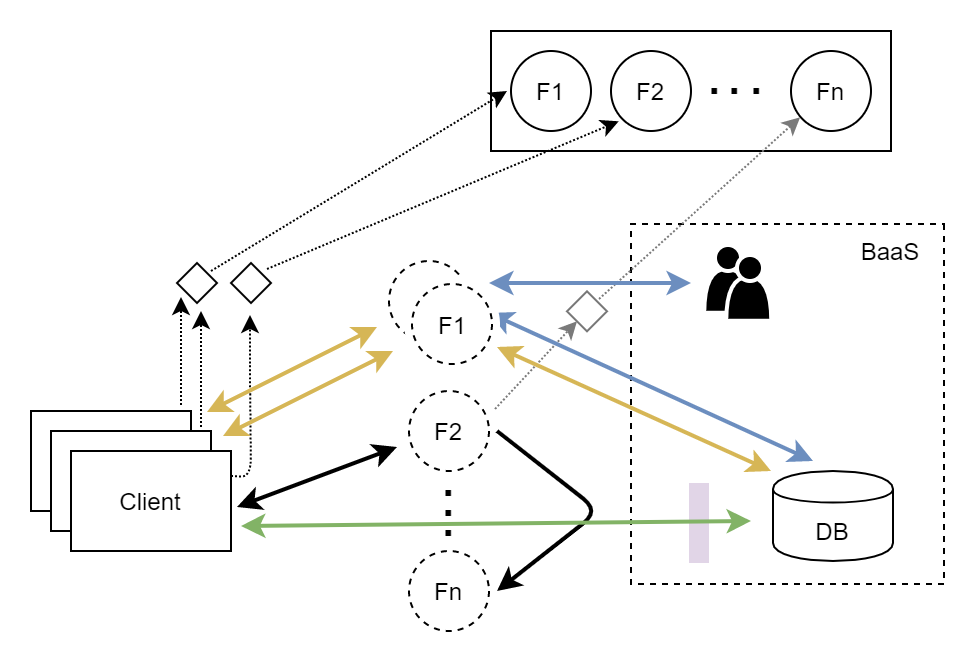
\includegraphics[width=0.7\textwidth]{FaaS}
\end{figure}
The function being called can either process the incoming request directly and return the result to the client or can access underlying BaaS services during the process of processing, as seen with F1. The services accessed and activated by a function can range from simple database queries up to register a new user, saving his profile data and provide certain permission to. The possibilities are only limited by the service ecosystem of the respective provider. Just like calling another function, the developer can also chain several functions to return the desired output. Chaining is only limited by the provider's orchestration solution and the maximum number of functions. \\\\
To better and more uniformly define FaaS and thus create a cross-platform standard, there is a growing demand in industry and research for a reference architecture such as that available for cloud or grid computing \cite{liu2011nist}, \cite{foster2003grid}. The absence of such an architecture hinders the establishment of best practices, design patterns and a more precise an overview of how the field of Function as a Service is developing \cite{leitner2019mixed}. Initial suggestions for what the reference architecture of FaaS might look like have already emerged. Reason to that is increasing popularity of FaaS in research and literature over the years, starting in 2016  \cite{van2019spec}. While the topic was not addressed until 2016, the presence of FaaS has been increasing continuously from then until 2019, in journals, conferences and workshops \cite{Yussupov2019_SystematicMappingStudyFaaS}.


\subsection{Dissociation of FaaS and Serverless}
Serverless computing, often referred to as serverless, is a sub-discipline of cloud computing that has evolved from the virtualization of computing power, storage and networks \cite{jackson2018investigation}. As often, it is not easy to differentiate or distinguish between newly developing technologies. Initially, serverless stood for applications which partially or completely relied on third-party providers, on so-called Backends as a Service (BaaS) [see Figure ~\ref{fig:serverlessBaaSandPaas}]. To perform server-side tasks such as database queries, user administration, Push-notification and other typically used web- and app-functionalities, the different vendors provide a vast service-ecosystem to fulfil those needs \cite{fowler2018serverless}.\\\\
With FaaS, the serverless concept has been extended so that the server-side logic is no longer completely provided by a third party. With FaaS, the developer has the possibility to execute business logic as a middleware between the client and the backend. This logic can be implemented by the developer himself. Serverless is one of the most frequently used buzzwords in IT in the last few years, whereas the term \glqq serverless\grqq{} suggests something different than what it actually is. The term implies the absence of servers, which is true from a physical perspective but not in regard to the responsibilities. In the broadest sense, serverless means a shift of responsibilities and operational tasks. Developers of a serverless application, do not have to deal with the operational activities such as provisioning, monitoring, maintenance, scalability and the robustness of the infrastructure \cite{baldini2017serverless}. However, the transfer of responsibilities is only possible with a certain degree of vendor lock-in, whereby the providers ensure that with FaaS, many services, provided by their ecosystem are used in conjunction \cite{kritikos2018review}. As many triggers as possible, presented in the previous section, should be used when building serverless applications.\\\\
Function as a Service is thus largely derived from Event-Driven Computing, which is used primarily in UI development and has been adapted by serverless computing. Nevertheless, the term serverless is equated with FaaS in many cases, loudly in 58\% of the cases studies by Leitner et al., which makes it difficult to distinguish between the two \cite{leitner2019mixed}. Figure ~\ref{fig:serverlessBaaSandPaas} illustrates the relationship between the different concepts.
\begin{figure}[H]
\caption{Serverless Concept, including FaaS and BaaS}
\label{fig:serverlessBaaSandPaas}
\centering
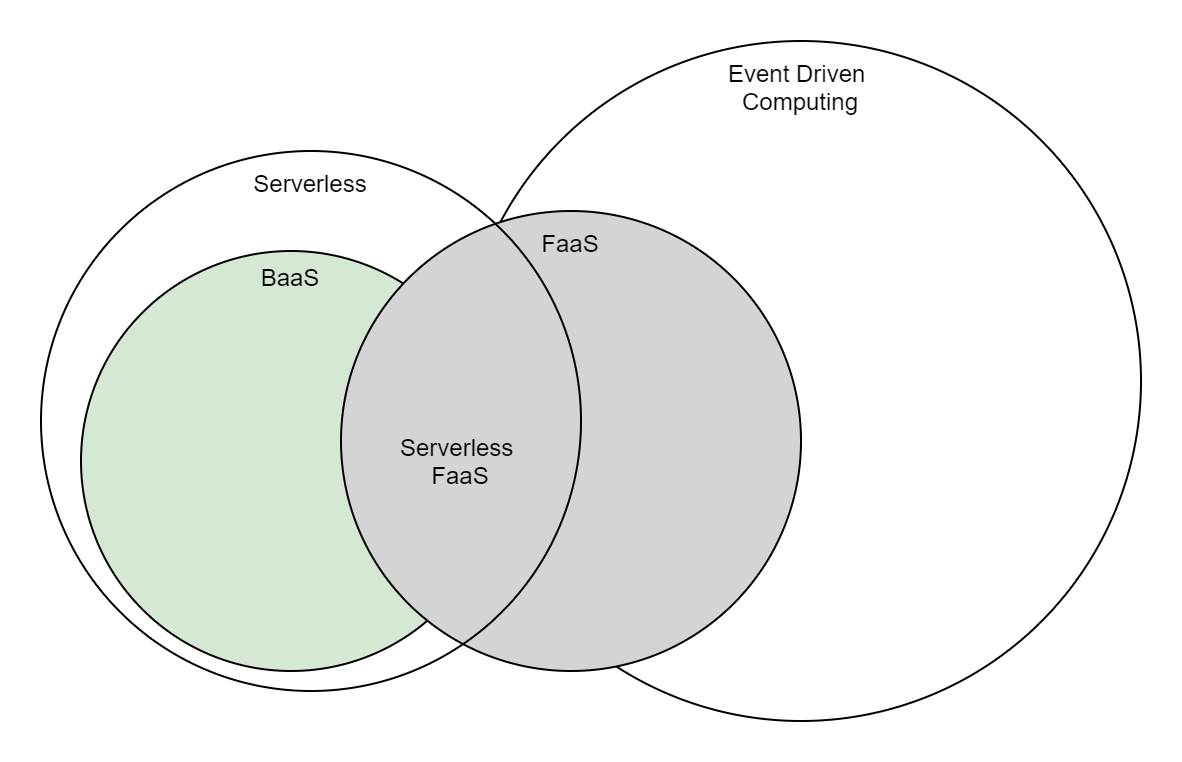
\includegraphics[width=0.7\textwidth]{Serverless}
\end{figure} 
If an application subsequently consists only of the two previously mentioned serverless components, FaaS and BaaS, a distinction is often made between a \textit{pure serverless} application, i.e. an application whose operational part has been completely outsourced to a cloud provider, and a \textit{hybrid serverless} application \cite{leitner2019mixed}. In the latter case, the functions often act as glue. Tasks that run very frequently and most of their time are running IDLE, do not claim any CPU or memory and as a consequence are not charged for. In IaaS and PaaS, these tasks probably run in a separate container, and therefore permanently are running. \\\\  
It has to be mentioned that a large part of the infrastructure-related tasks is also performed by the cloud provider when using PaaS. However, FaaS goes a step further at this point. With Paas, pre-built packages of an application are provided on the runtime of the corresponding platform, so the developers still have to take care of the application structure \cite{kaplan2019framework}. In FaaS, however, those tasks are performed by the platform provider and the developer can concentrate solely on the business logic and the respective event triggers. \\\\
Finally, the frequently used term \glqq NoOps\grqq{} \cite{fowler2018serverless} should be addressed, that mistakenly implies the absence of operational tasks. Although a large part of the maintenance is outsourced, this is not to be equated with the assumption that the operations of DevOps will be discontinued, as is suggested \cite{fowler2018serverless}.  Though the cloud-vendor handles load balancing, automatic scaling, security aspects and software patches, other tasks still need to be addressed by the developers and operators. It is still up to the developers to write high-quality code and test it locally as well as in the cloud environment to ensure its performance. The complexity is, therefore, not completely eliminated but shifted to a certain extent \cite{eivy2017wary}. Looking at AWS, a large number of configurations must be made, to properly and securely operate in production.\\ Starting with configuring the AWS API-Gateway, for being able to shift traffic for, i.e. testing purposes, the IAM needs to be configured afterwards. Furthermore, there is not one IAM to be configured but several, depending on the amount and type of functions as well as other services used on AWS. Although existing configuration, once made, can later be applied to other functions, it is essential to carefully configure them, to not run into security problems in a frequently used multitenancy environment.


\subsection{Benefits and Drawbacks}
Die im Folgenden aufgelisten Potential und Herausforderungen, denen sich Literatur und Anwender von FaaS gegenübersehen, sind zu Teilen dem Konzept selber, zu Teilen aber auch der Implementation der jeweiligen Anbeiter bzw. Open-Source Lösungen geschuldet. Es werden daher auf Seiten der Herausforderungen diese zunächst erläutert und falls in der Literatur bereits adressiert, vorgeschlagen Lösungen aufgezählt. Bei beiden, Potentiale und Herausforderungen, wird sowol Bezug auf FaaS als auch auf BaaS genommen, da diese beieden Kategorien in den meisten Fällen in Kombination genutzt werden bzw. architektionisch beding stark korrelieren [siehe Abbildung ~\ref{fig:serverlessBaaSandPaas} und \glqq statelessness\grqq{} Abschnitt \textit{Function as a Service}].\\\\ \\
\textbf{Cost efficiency}\\
A very frequently mentioned benefit of serverless computing and especially FaaS, is its const efficiency \cite{lee2018evaluation}. By only paying for compute time and memory size allocated to a function, the amount of functions store on the platform do not matter to the developer. In addition, the event-driven nature of FaaS and the remote runtime provisioning, solely when an event triggers the function, are critical for cost efficiency \cite{feng2018exploring}. Even though the cost efficiency of FaaS can be a huge benefit for some use cases, FaaS is not an ideal solution for all use cases. When functions run over a long period and get triggered very frequently, PaaS solutions are likely the better choice. The price for executing a function then runs for one minute is generally lower then executing the same code on a PaaS server with similar resources \cite{jonas2019cloud}. Looking at PaaS, the primary purpose is to execute functions that experience permanently high demand, functions are primarily intended to solve simple, high-traffic tasks where the user only has to pay for the resources that the function uses when it is called. Pikes do not need to be recorded to adapt the memory or computing size of an application running in a PaaS hosted container. No adjustments need to be made based on historical data. Nevertheless, Elgama et al. exhibit, that also with Function as a Service the need to decomposite functional components of an application is still required, even in regard to the pay-per-use model. Not separating functionalities effectively into separate FaaS functions with different memory can disadvantageous influence costs \cite{elgamal2018costless}.\\\\ 
\textbf{Time to Market / Lead Time Development}\\
Tough lead time developemnt is not the primary benefit of using FaaS, it is mentioned in several papers as being on of the key benefit serverless enables \cite{adzic2017serverless} \cite{ast2017self}. According to Leitner et al. Time to Market is not one of FaaS primary advantages, which is according to the study the scalability and elasticity \cite{leitner2019mixed}. With FaaS it is possible to deploy code within seconds and minutes. In regard to different testing approaches, such as canary releases, many cloud vendors, such as AWS, provide simple predefined solutions for such purposes. By utilitzing services such as API gateways, the platform supports fast developemnt and deployment. Changes can be quickly made to a functions and tested individuall in the cloud \cite{sewak2018winning}.\\\\
% \textbf{Optimal Utilization of Data Centers}\\
% Greener Computing \cite{shafiei2020serverless} \cite{fowler2018serverless}
% \\\\ 
% \textbf{Vendor Lock-In}\\
% The vendor lock-in is neither a benefit nor is it a drawback and depends on the purpose it FaaS is introduced for. \\\\
\textbf{Physische Lokation}\\
Another point to consider is the physical location of the functions. It is the provider's responsibility to use its resources as efficiently as possible. Therefore, he decides on which node in his infrastructure a function should be executed. If the provider subsequently locates functions that are highly data-dependent physically far apart from each other, effects on performance are more likely to be faced by the users of the application \cite{shafiei2020serverless}. Although many providers, such as AWS, Microsoft or Google, already offer the option of defining the region or a so-called cluster, this only allows the location of the function to be limited to a certain area, but not to exactly define the server the functions should be executed on. FaaS cannot match the performance of serverfull applications \cite{shafiei2020serverless}.\\\\
\textbf{Serverless}\\
At this point, it might seem relatively trivial, but still, a disadvantage compared to solutions like PaaS or IaaS. We are talking about the loss of server-side optimization. As the name already implies, servers do not exist for users or, in the case of a software solution based on BaaS, the developer has no control over the backend. He can only adapt the databases, object storage or authentication to the structure of his data and implement access restrictions via rules. The services are predefined by the respective vendor and cannot be adapted to the corresponding client types, such as a tablet, mobile phone or desktop. They can not be optimized to meet the requirements of the \glqq Backends For Frontends\grqq{} pattern, written by Sam Newman\footnote{https://samnewman.io/patterns/architectural/bff/}. The topic of only one BFF-service for multiple clients is further discussed by Perera et al. in \cite{perera2018rule}. There is only one version of each type (databases, object storage, authentication, and so on) to which developers are restricted. Any user-defined logic must, therefore, be outsourced to the client, as it cannot be implemented on the backend side \cite{fowler2018serverless}. With FaaS, this effect can be mitigated by implementing lightweight logic in the form of functions, that act as middleware on the server-side. This involves interacting with the various BaaS services, using the triggers provided by the cloud vendor [see section \textit{Function as a Service}].\\\\ 
\textbf{Statelessness}\\
The statelessness of functions, on the one hand, enables the pay-per-use model and scale-to-zero functionality of FaaS, but on the other hand, presents a problems practitioners have to deal with. The core of applications is to solve tasks that require many different steps which need to be connected in a meaningful way, in order to provide the desired output. Thus, even with the function-based structure of applications, it is essential that the functions can intercommunicate and query the program status from each other without inconsistencies. Due to the short runtime of functions, the exchange of information must take place at a corresponding speed. However, as pointed out in a report from Berkeley, fast and accurate state sharing still proves to be problematic when considering the speed of serverless applications compared to serverfull applications \cite{jonas2019cloud}.\\\\ 
To persist the state of an application, the Key-Value-Storages and object storages offered by the providers can be used. Object storages of the different providers (AWS S3, Google Cloud Storage, Azure Blob Storage) are not very expensive in terms of storing data, but the costs for accessing the storage are high and the latency of up to 20ms is high too \cite{jonas2019cloud}. The key-value storages are the better choice in this case, as their response times are lower with 8 - 15ms, but they are significantly more expensive than object storages, in terms of their input/output operations per second \cite{jonas2019cloud}.\\\\ 
Taking the neccessity of fast exchange of information, between functions and external storage mediums, into account, it might be more appropriate to pass a functions state, when interconnecting functions, form one function to another without querying the current state form an external database. As mentioned above at the \textit{physical location} of functions, it is likely that functions are not started on the same node. The load balancer of the respective provider decides on which node a copy of the function is executed, depending on the current load on the infrastructure. Even though in a perfect world, the transfer of the application state is faster when interconnecting functions than querying a database, the advantage is mitigated by factors inherent to FaaS. Those factors are not inherent to the concept itself but to the technical implementation.\\ As a consequence, the effect of fast state transfer between functions is relativized by the functions startup latencies and physical distance from each other, which can not be influenced by the developer. To counteract this, Shafiei et al. suggest marking interrelated functions to draw a dependency graph and starting possible subsequent functions directly at the initial call of the first function \cite{shafiei2020serverless}.\\\\
If the user were allowed to determine on which instance (node) a function should run, the concept of FaaS would be undermined (see \textit{Optimal Utilization of Data Centers}). Enabling developers to precisely choose the instance a function-pool should run on capacity would need to be reserved for those users. The provider would have to hold the capacity back, in order the functions, specific to a user, are called. The vendor would no longer be in charge of its platform and could not free unused capacity to other users in order to increase efficiency [see \cite{fowler2018serverless}]. 
\begin{figure}[H]
\caption{Dependency Graph nach \cite{shafiei2020serverless}}
\label{fig:dependencyGraph}
\centering
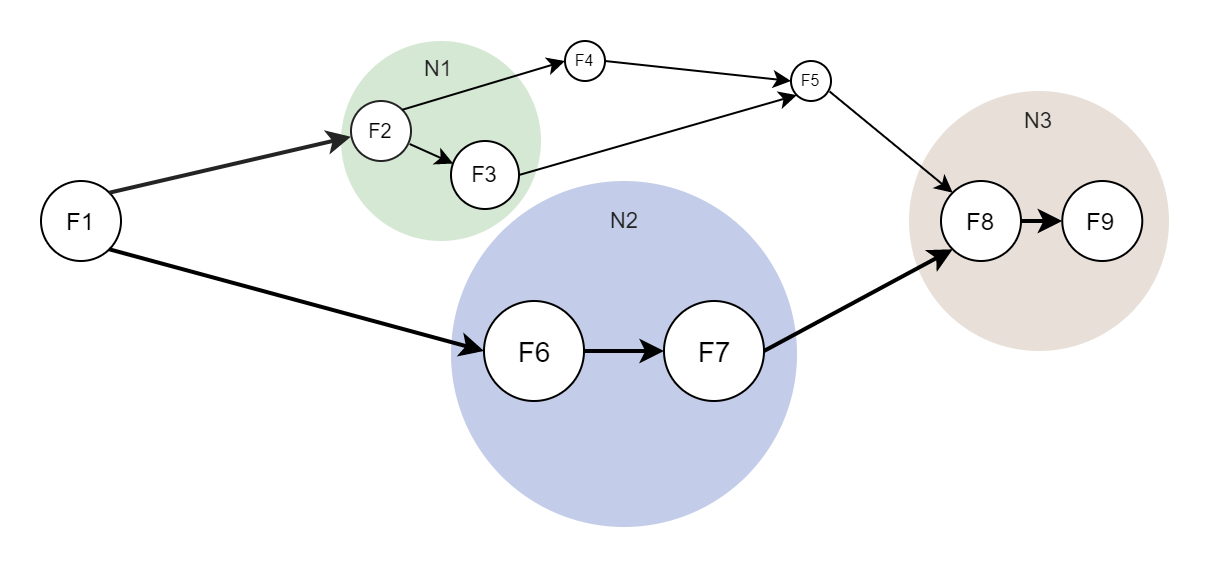
\includegraphics[width=1\textwidth]{DependencyGraph}
\end{figure}
If each user could determine on which node, e.g. Node-X, his functions should run on, in order to pass on the program status with as little physical latency as possible, an optimal workload could no longer be guaranteed. The provider would always have to retain capacity from Node-X and could not release it for other functions. He would always have to retain some part of the capacity of Node-X in case inactive functions are allocated. A dependency graph, as shown in the figure ~\ref{fig:dependencyGraph} would bypass the need of determining a specific node. Specifying a node would no longer be necessary, since the provider could start functions, connected via the dependency graph, simultaneously. With the time of cold starts and dependency instantiation saved, the only the physical location of the functions could affect latencies. The provider's load balancer could be able to start functions as usual. Since latencies when starting a service are considerably higher than those caused by the location, their elimination would considerably accelerate the state propagation \cite{aditya2019will} \cite{jackson2018investigation}. In addition, the language used for the function will influence its startup latency as well. Therefore object-oriented and functional programming languages should be weighed against each other \cite{manner2018cold}. \\\\
By combining this approach, which already accelerates intercommunication, with a simple neuronal network, predictions on functions could be made. Looking at figure ~\ref{fig:dependencyGraph}, by weighting the edges connecting the nodes, the probability of hitting F2 instead of F6 could be further determined. Thereby the platform could use their resources even more effectively because not all functions connected in the dependency graph would have to be started. However, if the prediction is in favour of F2 but F6 is triggered, then the latency, caused by ist cold start, could increase, but also changes to the edges of the graph would be made.\\\\
\textbf{Multitenancy}\\
Although the concept of FaaS is based on the fact that the provider controls and maintains a variety of functions from different customers, each customer should feel as if they are the only one. However, this poses additional challenges on the platform operators, as they must reliably guarantee resource isolation and access restrictions. Even though the providers manage to guarantee resource isolation reliably, the user still has to set up his security rules properly.\\ Conditioned by the nature of serverless applications, they are based on the communication and interconnection of services and functions. For each function, a security policy needs to be set up. If the policy is not configured correctly, this already represents a security risk. The functions and services could grant access to data, which was not intended by the user \footnote{https://awsinsider.net/articles/2017/06/20/voter-data-leak.aspx},\footnote{https://searchsecurity.techtarget.com/news/450422962/Another-AWS-cloud-data-leakage-due-to-misconfiguration}.\\\\
Although providers like AWS should be experienced enough by now not to expect such problems anymore, caution is still required \cite{fowler2018serverless}. They constantly have to deal with security, robustness and performance of their infrastructure. No customer should see another's data, no error should compromise the stability of other functions, and no sudden spike from one customer should affect the performance of another's customers functions. The interaction between RPCs and container security must be permanent and be ensured by careful security management \cite{mcgrath2017serverless}.\\\\
\textbf{Cold-Starts}\\
Cold starts refer to starting a container in which a copy of the required functions is provided. If a function has not been used for a long time or is being addressed for the first time, everything needs to be prepared for execution at first. Especially with very short functions, they pose a considerable problem, since their start-up time can be up to ten times the actual execution time \cite{shahrad2019architectural}. A container must be started on a node and the function and its dependencies have to be loaded. The time it takes for the instance to be ready for porcessing a request, depends on various factors. Factors can be the programming language, the required libraries, the size of the function (amount of code) and the hardware on which the function is instantiated \cite{shafiei2020serverless} \cite{jonas2019cloud}. If a function is called very frequently, the platform keeps these functions \glqq warm\grqq{} for a certain time (up to one hour for AWS \cite{roberts2017serverless}), so that the probability of a new cold start tends towards zero. In contrast, functions that are called only once per hour are more likely to experience the effects of cold starts, each time they are accessed \cite{roberts2017serverless}. \\\\
To counteract this, Castro et al. propose to keep a kind of stem cell container. The container would hold already instantiated but empty containers for the supported programming languages \cite{castro2019server}. The containers are not customer specific and can therefore be used generically. This would eliminate two of the above mentioned issues the programming language and the hardware, which negatively influence the startup time of the functions. Only the business code of the functions and their dependencies need to be loaded. Ishakian et al. have also shown that by increasing the memory capacity, the time until a function is ready to process a request, can be reduced \cite{ishakian2018serving}. If this is combined with the stem cell approach, the loading of the program code and its libraries is accelerated. Of course, the additional memory does not come for free, but in this case it is up to the company to weigh the additional costs against the performance increases.
 \newpage
 %Keep alive \cite{lloyd2018improving}





\section{Guideline on Migration}
The below-presented guideline for migrating parts of existing microservice architecture to the relatively new cloud-computing concept, Function as a Service, is structured as follows. At first, the decision to migrate is questioned by challenging the motives of adopting this new technology and giving advice on when to migrate. Afterwards, criteria for selecting the right service will be stated. Those criteria gear towards the possibilities that come along with FaaS. When a reasonable service has been found, a provider needs to be identified, which best meets the company's requirements. There are two types of providers that primarily differ in the service-ecosystem inherent to them and the degree of vendor lock-in. Whereas proprietary platforms like AWS, Azure, or Google provide a vast ecosystem of feature services and Backend as a Service offering, open-source frameworks like OpenWhisk, Fission, OpenFaaS or Kubeless dedicate greater control to developers. When implementing FaaS, the open-source solution can be far more adjusted and configured to best suit an organization's needs. Next, impacts on the general process of software development will be investigated. Changes in an organizational structure regarding the development team, effects on the CI/CD pipeline, challenges faced with local testing and the VCS, will be addressed. At this point, it should be outlined, that this thesis differentiates between the testing that is done locally during development and testing, which needs to be done on the ecosystem of the platform itself. With the development process covered, the guideline on migration will end with the operational part. Alternations on the process of monitoring, maintenance, and testing instances will be covered, and advice on coping with them will be given.\\\\ To better follow along with the guideline, the subsequent section will provide an overview of the current microservice infrastructure. The development process, as well as the operational tasks, will be described, along with the underlying service-landscape. Ending with a summary on the constructed guideline, changes affecting the current infrastructure will be outlined.
\subsection{Describing the existing architecture}
In the afterwards, the current process of development and operations is described, to later on better illustrate the effects of introducing Function as a Service to the existing microservice architecture, see \cite{newman2015building}. Figure ~\ref{fig:devopsone} provides a high-level overview of the prevalent DevOps-Pipeline. In the final stage of this section, by summing up on the construction of the guideline, figure ~\ref{fig:devopsone} will be examined regarding necessary changes.\\\\ Starting with the development team, it consists of around eleven developers that are working after Scrum, an agile process framework,see \cite{pichler2013scrum}. During a sprint, the team splits up in groups of two to four, to work on the tasks they committed on. Thereby the primary language used for developing the services is Java. Following a typical pattern, the basic structure of a service is defined in a YAML-file \footnote{https://yaml.org/}. In this file configurations regarding the endpoints of a service, its request and response parameters and other basic configuration can be made. The YAML-file then gets passed to swagger-codegen, which generates a service skeleton with the according interfaces. Using Maven as an automation tool for service development, when building the service, all required dependencies, specified in the POM, will be loaded. The POM itself is an XML-file, including information about the service. The file documents target locations, dependencies, versions and other default configurations for building the service. After the initial build of the service, the business logic can be implemented. To keep track of different versions of services as well as the entire service landscape of the platform, a VCS like Github, Bitbucket or Tortoise can be used. While working on the business logic, the service will be built and tested several times. The tests are executed in the local development environment, using mock data form test-databases. By the time the service is documented, a PR can be created. To guarantee a certain service-quality, all services embrace parts of a so-called core-service. The core-service enforces certain standard functionalities in terms of logging, messaging, caching, circuit breakers, standard exceptions and many other tasks, other services have to incorporate. Given that the service implements the standard correctly and the code-review reveals no flaws, by approving the PR, the CI/CD pipeline is triggered.     
\begin{figure}[H]
\caption{DevOps Pipeline}
\label{fig:devopsone}
\centering
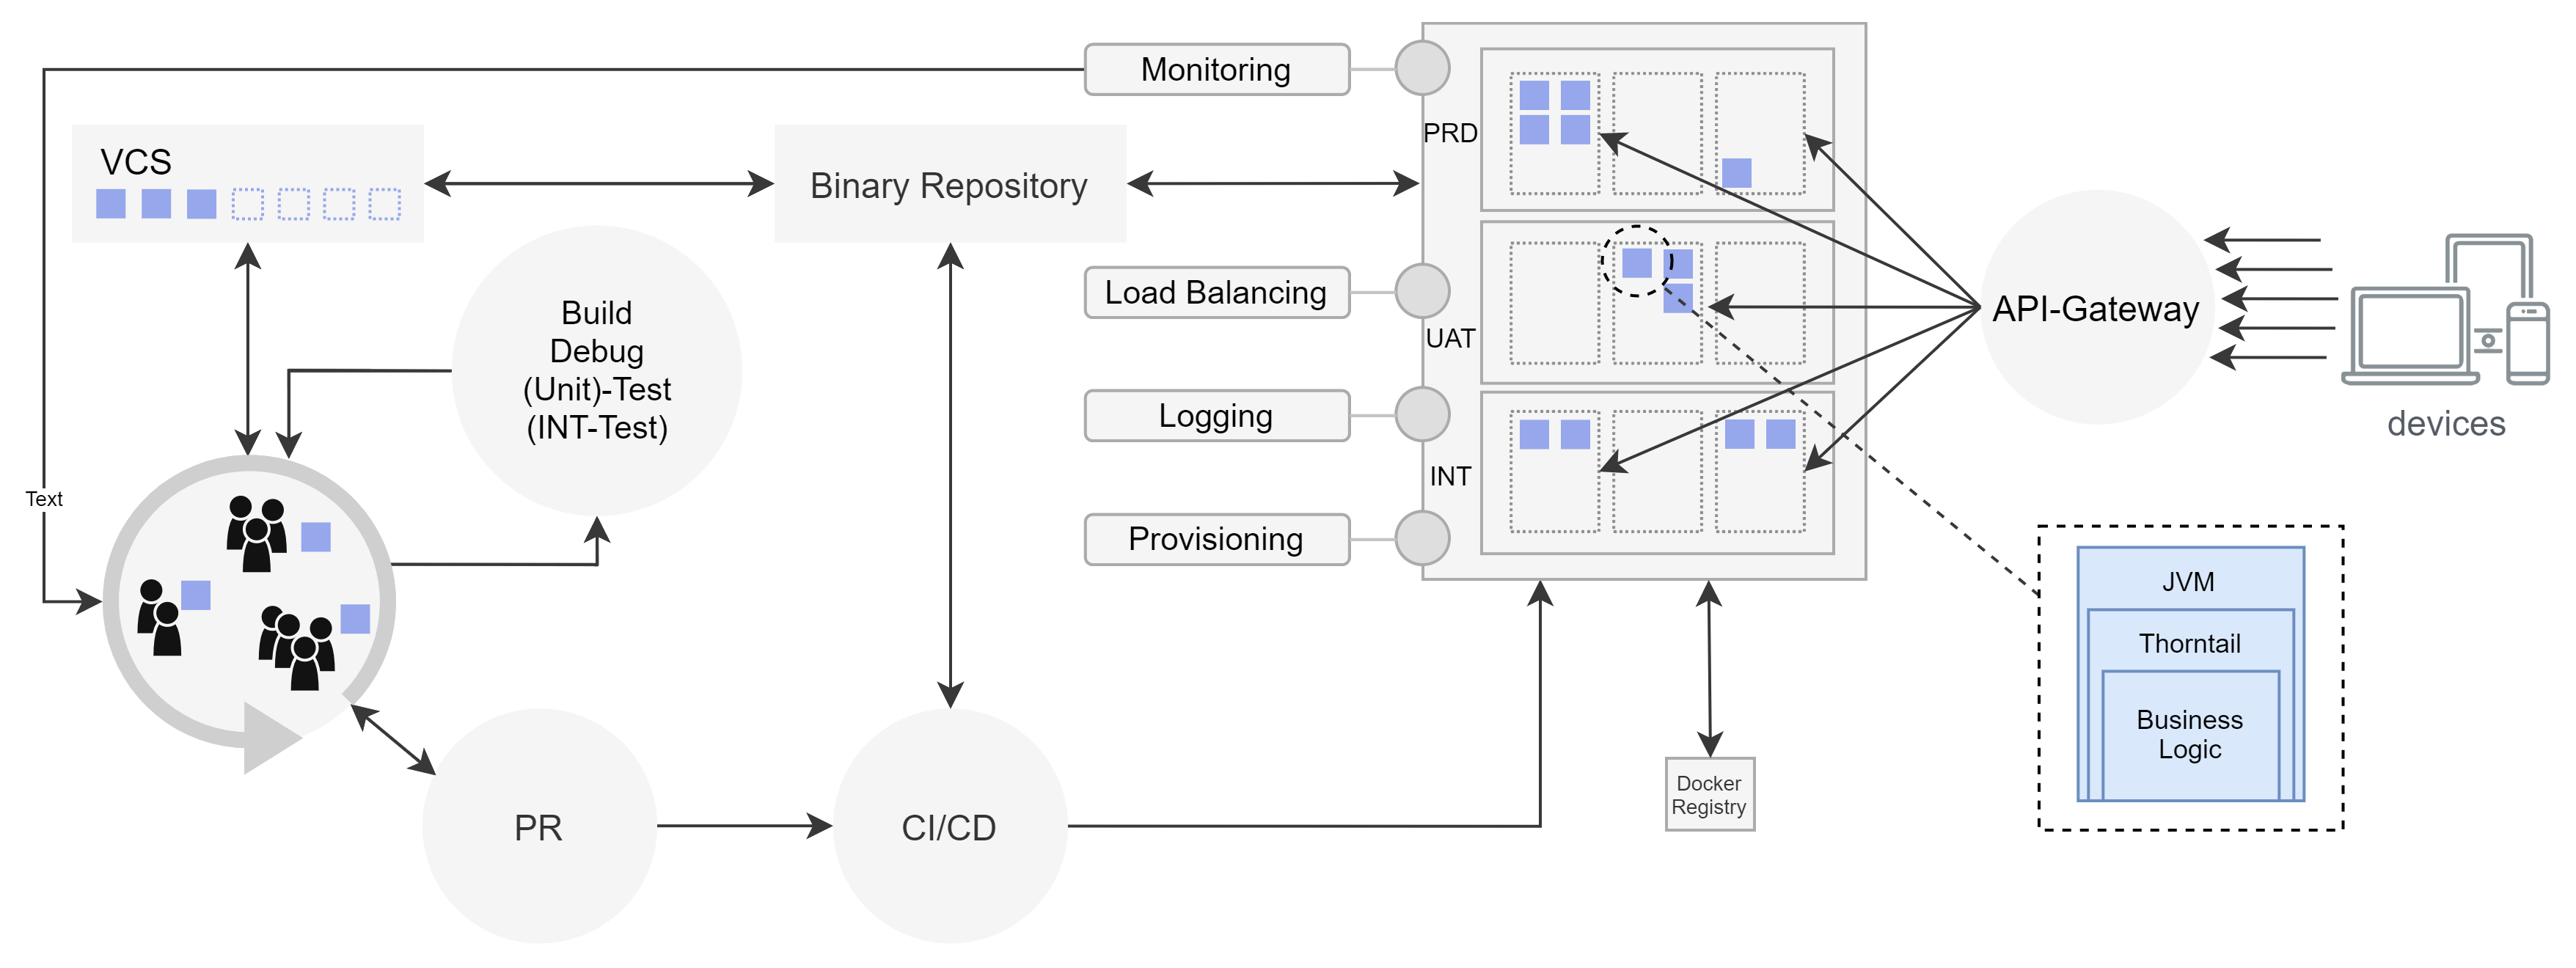
\includegraphics[width=1\textwidth]{devopsone}
\end{figure}
Looking at the CI/CD pipeline, different products can be used for automation. Two popular choices are Jenkins and TeamCity. The purpose of the pipeline is to build a service, execute tests, and provide the services war-files and jar-files to a binary repository. The binary repository itself is connected with the VCS as well as with the CI/CD pipeline. By triggering a build process for one of the services its binaries as well as complementary program parts -- such as Git, the JVM, Thorntail etc. --, will be put into a Dockerfile. Based on the Dockerfile, a baseimage will be built, containing all specified programs that are needed for the program to run correctly. This baseimage will be forwarded to a container where the application runs on in the end and is stored in the Docker registry for later usage. When a new instance of a service is needed, it can be loaded directly from the Docker-registry. To ease working with containers, Kubernetes was installed, which is an open-source framework for automating deployments, scaling and management of containerized applications.\\\\ Microservices are usually hosted on-premise, PaaS or IaaS solutions and run in a container. A pre-defined amount of memory and computing resources are allocated to a container, enabling it to handle a certain magnitude of incoming traffic. When the traffic exceeds a predetermined threshold, another instance of the service will be provided on the platform, using the baseimage from the docker registry. Due to the horizontal scaling nature of containers, each instance has a fixed amount of resources which are constructed to deal with incoming traffic.  In practice, the containers are running most of the time in IDLE. Even though microservices already have decoupled many monolithic applications into smaller, more manageable systems, they still incorporate different functionalities. In reality, microservices can get quite large and therefore need to be grouped by bounded context to better suit the concept of FaaS. Because of their size, it takes time to launch a new container, in case the incoming traffic rapidly increases. Therefore it is good practice to provision at least two service instances if historical data has shown frequent bursts in load. 
\subsection{Scrutinising the Decision of Migration}
Whereas migrating from a monolithic application to Function as a Service seems far more challenging, due to the assumed size and complexity of the monolith, migrating from a microservice architecture to FaaS can be challenging as well. With a monolithic application, partitions need to be identified in the first place and afterwards be broken down into small services. Microservices, on the other hand, might already be small enough that they supply only certain functionalities. Still, in some cases, they do incorporate too many functionalities to be converted to functions right away. Nevertheless, issues that have to be dealt with will remain. When migrating, a solution for outsourcing the internal state of the microservice has to be taken into account. Furthermore, dependencies need to be reduced to a minimum and the code probably has to optimized to suit the concept of FaaS better.\\\\ Before starting to introduce this new technology into the service landscape, it is essential to contrast the current state of the system with the desired state. When a system is already composed of many small services, the underlying infrastructure likely consists of VMs or containers. Those containers often run in a PaaS environment, and it is not possible to scale them to zero to free reserved computing capacity, in favour of other services to consume it. To do so or even to outsource the expense of provisioning services, managing the underlying infrastructure and coping with operational tasks, such as monitoring, load balancing. Function as a Service can help to achieve this desired state. The restrictions that come along with the ease of development have to be traded off against its benefits.\\\\ To profit as much as possible of introducing FaaS, the services, which should be migrated, have to be inspected regarding dependencies, size, version, language, and complexity. It is recommended to reduce dependencies to a minimum, due to their effect on start-up times \cite{manner2018cold}. Especially with Python, Nodejs, and Java \cite{puripunpinyo2017effect}, loading all dependencies required can have an impact on cold starts. Also, the dependencies might again interconnect with other dependencies, resulting in a considerable number of dependencies, that should not be underestimated. With FaaS, each unnecessary dependency will increase the start-up time of every single Function being started.\\\\ The next issue which needs to be addressed is state management. As mentioned in section two, \textit{benefits and drawbacks}, there is no persistent state an application can rely on. Being precise, there is a persistent state in the container of a function, but whether an incoming request will hit a particular container, is unpredictable. When a service does not receive any request or is running for a long time, the provider will eventually kill its container to free capacity. In the case of AWS Lambda, the current maximum amount of time, of a frequently called function until it gets killed, is 45 minutes\footnote{https://aws.amazon.com/de/lambda/}. Later on, when comparing cloud providers with open-source frameworks, there will be guidance on finding an appropriate solution to meet a company's purpose. Still, for now, the following must be considered. When using an open-source framework like OpenWhisk, the external state management system can be covered with Redis or another low latency database. Whereas using a cloud provider platform, one of its integrated database solutions will presumably be the best choice. If it is necessary to have full control over the performance and configuration of the database, an open-source framework has to be chosen.\\\\ The latency and frequency of a service will also decide upon its aptitude for being a candidate to get migrated to FaaS. If the service is called very frequent and experiences most of the time very high traffic, the concept of Function as a Service will not apply to it \cite{jonas2019cloud}. Due to a limit of concurrent running functions, that can vary between the different providers and frameworks; incoming traffic can only be handled upon a certain amount. Moreover, the same application experiencing the same vast amount of traffic, once running on a FaaS platform and once running in a docker container on PaaS, will be more expensive implemented with FaaS, than it will be with PaaS \cite{jonas2019cloud}. Therefore, services with various workloads, having eventually high peeks and then some time of inactivity, are more applicable to the concept of serverless, than their counterparts.\\\\ Latency should also not be a critical component of the system due to the before mentioned cold starts. Latency sensitive applications like trading platforms, which strongly rely on real-time data, are not a suitable candidate for Function as a Service. Another pitfall is the promise of not having to maintain, provision, scale, or monitor the infrastructure and thereby reducing complexity and operational tasks. On one side, the cloud provider will, to some extent, take care of load balancing, scaling, provisioning, versioning and providing monitoring solutions. On the other side, new complexity will appear in other areas. To cope with the complexity given by a potentially large number of functions, the issue of mono-repo and poly-repo arises, as discussed in a later section.\\\\ Lastly, attention needs to be drawn to the programming language and lead time development. FaaS can provide a reduction in lead time development and time to market, thanks to its small codebase and rapid development \cite{sewak2018winning} \cite{leitner2019mixed}. Developers can make changes, fix issues, test, and finally deploy a new version to production in a view minutes. Prerequisite, even though this might sound trivial, is the language support for the language used in the application or service. If the platform does not provide the required language, to avoid the hassle of finding a workaround, an alternative solution should be chosen. Although the big cloud providers already support many programming languages, application logic might have to be rewritten, if that specific language is not supported. In the case of version incompatibility, parts of the application needs to be rewritten as well. Especially when the provider's version is below the version of the application, it becomes an issue.
\subsection{Balancing between Open-Source and Cloud-Vendor}
Choosing an open-source over a cloud vendor, or the other way round, depends on the purpose of utilization. Neither is the so-called vendor lock-in a drawback nor a limitation, compared to an open-source solution; it is solely a tradeoff between the benefits of two different approaches of the same model. Nevertheless, the decision on one of them will affect the possibilities in the process of development and migration. To answer the question on which one to choose, the following things need to be considered.\\\\ If the primary purpose is to start rapid development with not having to configure any infrastructure, a cloud vendor seems to be a promising solution, especially when a project has no legacy application that needs to be refactored or rewritten. Which vendor should be taken is dealt with in the following section.\\\\ With Amazon Web Services (AWS) Lambda, Microsofts Azure Functions, IBM Cloud Functions or Google Cloud Functions, each of the large serverless providers has a considerable amount of services in its ecosystem. The ecosystem is utterly compatible with itself, making the need to find a custom workaround for processes like CI/CD obsolete. AWS and Azure even provide a premade solution for that purpose. Moreover, if an application requires user authentication, different types of databases, messaging services and hosting, each of the platforms can satisfy these needs. Adding to that, they provide an appealing pricing model with free contingents each month, which makes them a feasible candidate for experimenting with different cloud services.\\\\ Unfortunately, these benefits do not come without restrictions. By ceding the responsibility of provisioning, load-balancing, scaling, error-handling, monitoring and many more duties to the cloud provider, one is dependent on the tooling provided by the platform. Just because the responsibility of maintenance and provisioning is outsourced to the provider, this does not mean that there is no need for an additional monitoring practice, as later stated in \textit{implications on monitoring}. In case something goes wrong on the platform, it is recommended to have, besides the tools offered by the provider, additional information to rely on. To reproduce the error, the custom logging data can be crucial to find the cause of the problem and solve the problem.\\Another point that has to be considered is the outage of the platform, which is per se not exclusively a cloud provider issue, but something that might have to be dealt with. A possible solution to this is a framework sitting between development and the platform, enabling multi-cloud application that can produce relief.\\\\ Depending on how one looks at it, Function as a Service in conjunction with Backend as a Service can be depicted as an advantage or disadvantage. Even though the two concepts undertake many tasks, for many tasks, additional services need to be consulted. E.g. when building a serverless application, for messaging an SNS-service, for storing the state a database-service, for registring new users an authentication-service and form monitoring a monitoring-service needs to be included. Not yet mentioned CI/CD integration, API-Gateway and many more.\\\\ If the concept of FaaS should be introduced to a company or project along with staying in control of the entire infrastructure, a cloud provider solution is not applicable. In this case, an open-source provider needs to be chosen. If the present application is built upon Kubernetes, for the purpose of virtualization, Kubeless, OpenWhisk, OpenFaaS and Fission are feasible FaaS options, that can be integrated with little effort \cite{palade2019evaluation}. Using an open-source provider, configurations in terms of computing time and resource capacity can be customized, due to being in control of the underlying platform. Introducing FaaS to an upfront ecosystem will increase its performance and efficiency by freeing unused resources. At the same time, an operations team will be needed that is in charge of implementing a monitoring solution and configuring the properties of the FaaS framework \cite{mohanty2018evaluation}.\\\\ Furthermore, the team needs to acquire new skills to configure security policies correctly, interconnect function with each other, define different triggers on functions, deal with concurrency setting \footnote{https://docs.aws.amazon.com/lambda/latest/dg/configuration-concurrency.html}, and many more aspects add complexity to new fields. If the company aims at reducing infrastructural complexities, then Function as a Service can provide support on the listed tasks, but when its primary purpose is to reduce operational efforts, as often suggested with the term \glqq NoOps\grqq{} \cite{eivy2017wary}, FaaS, again, is not the right choice.
\subsubsection{Open-Source Solutions}
Depending on the decision made in the previous section, there are various frameworks and platforms at choice. Below, several solutions for each approach are presented. Starting with open-source frameworks, Fission, Kubeless, OpenFaaS and OpenWhisk will briefly be introduced.\\\\ \textit{Kubeless} is a Kubernetes native serverless framework, being a straight forward extension for a Kubernetes API-Server. Kubeless itself has no API-Server and no data store to store any files, objects, binary data and other formats in. Since it is reusing everything from Kubernetes, Kubeless solely relies on the API-integration. To scale functions, Kubeless makes use of the Horizontal-Pod-Autoscaler included in Kubernetes. Depending on the runtime, metric data can be monitored with Prometheus.\\Regarding the deployment of new Functions, the API, ConfigMaps and Ingress are utilised\footnote{https://kubeless.io/}. Thus being built on top of Kubernetes, making use of its CRDs\footnote{https://kubernetes.io/docs/concepts/extend-kubernetes/api-extension/custom-resources/} to create functions, users, familiar with the Kubernetes-API, can process as usual. The language-runtime itself is encapsulated in a container image which will be set in the Kubeless configuration. A list on supported runtimes can be found on \textit{github}\footnote{https://github.com/kubeless/runtimes/tree/master/stable}. Each function will be deployed in a separate Pod, supervised by Kubernetes HPA. When a function is not used, the HPA will kill the pod to free capacity. Prerequisite is the deployment of the function with a CPU request limit. Depending on the runtime, metric data can be monitored by Prometheus.\\\\ \textit{Fission} is a serverless framework build on top of an underlying Kubernetes infrastructure. Just like Kubeless, Fission does not inherit a resource store and therefor depends on communicating with the Kubernetes API-Service, in order to get access to secrets and ConfigMaps. As well as the former, Fission supports a large number of programming languages. Also, CPU and memory resource limits can be configured, ceding great control to the developer. Two aspects which make Fission unique compared to the other three is, for one thing, its ability to define the number of pre-warmed pods and for another thing its richness of possessing a Workflow-System. Whereas the pool of pre-warmed pods can be utilized to mitigate the cold start issue, the Workflow-System makes it easier to handle an increasing number of functions. Besides that, the Workflow-System facilitates scheduling and executing more complex workflows [see \cite{kritikos2018review}]. In contrast to Fission, Kubeless uses event chaining to create workflows which makes it harder to maintain the workflow graph, when an application keeps on growing \footnote{https://docs.fission.io/}.\\\\ \textit{OpenFaaS} provides a so-called \textit{faas-provider} interface, letting it integrate with any provider that has implemented the interface. Currently, these providers are Kubernetes, Docker Swarm and \textit{faas-memory}. Each function will be packaged into a docker image and deployed via the OpenFaaS CLI. With its API-Gateway, OpenFaaS can respond to any event, and by making use of its auto-scaling functionality the min/max amount of replicas can be configured\footnote{https://www.openfaas.com/}.\\\\ Lastly, \textit{OpenWhisk} is a serverless framework which has initially been developed by IBM and is now backed by Apache. Because OpenWhisk was backed by a large company, its application model is often referenced in literature when the application model of other large cloud providers is indicated. It can be assumed that other vendors are using a similar concept due to OpenWhisk being provided in a large cloud environment \cite{van2019spec}. As an orchestration tool, Kubernetes can be used in conjunction with OpenWhisk, as well as IBMs Composer. As with the other three language runtime support here too, is quite large, ranging from Go over Java and Python all the way to Nodejs\footnote{https://OpenWhisk.apache.org/}.\\\\ In addition,  all four open-source frameworks natively support three different types of triggers, see figure ~\ref{fig:OpenWhiskProgrammingModel}], namely HTTP, Event and Schedule. Adding to that, Fission, Kubeless and OpenFaaS are written in Go, OpenWhisk in Scala. Concurrency testers on Kubless, OpenFaaS and Fission have shown that the latter framework with 2ms has the fastest response time of all three. Moreover, its response times are consistent regardless of the number of replicas present and the number of concurrent users \cite{mohanty2018evaluation}. The test was conducted with 1, 25 and 50 replicas. Kubeless and OpenFaaS experience an exponential increase in response time. Although the response time increases an is higher compared to Fission, OpenFaaS is showing a slight decrease in response time the more replicas are prevalent. Finally, Fission has a success ratio of 100\% in all three tests, whereas Kubeless and OpenFaaS are facing a slight decrease from one to four percent.
\begin{figure}[H]
\caption{Median response time for each serverless framework with (a) 1 replica, (b) 25 replicas, and (c) 50 replicas \cite{mohanty2018evaluation}}
\label{fig:opensource}
\centering
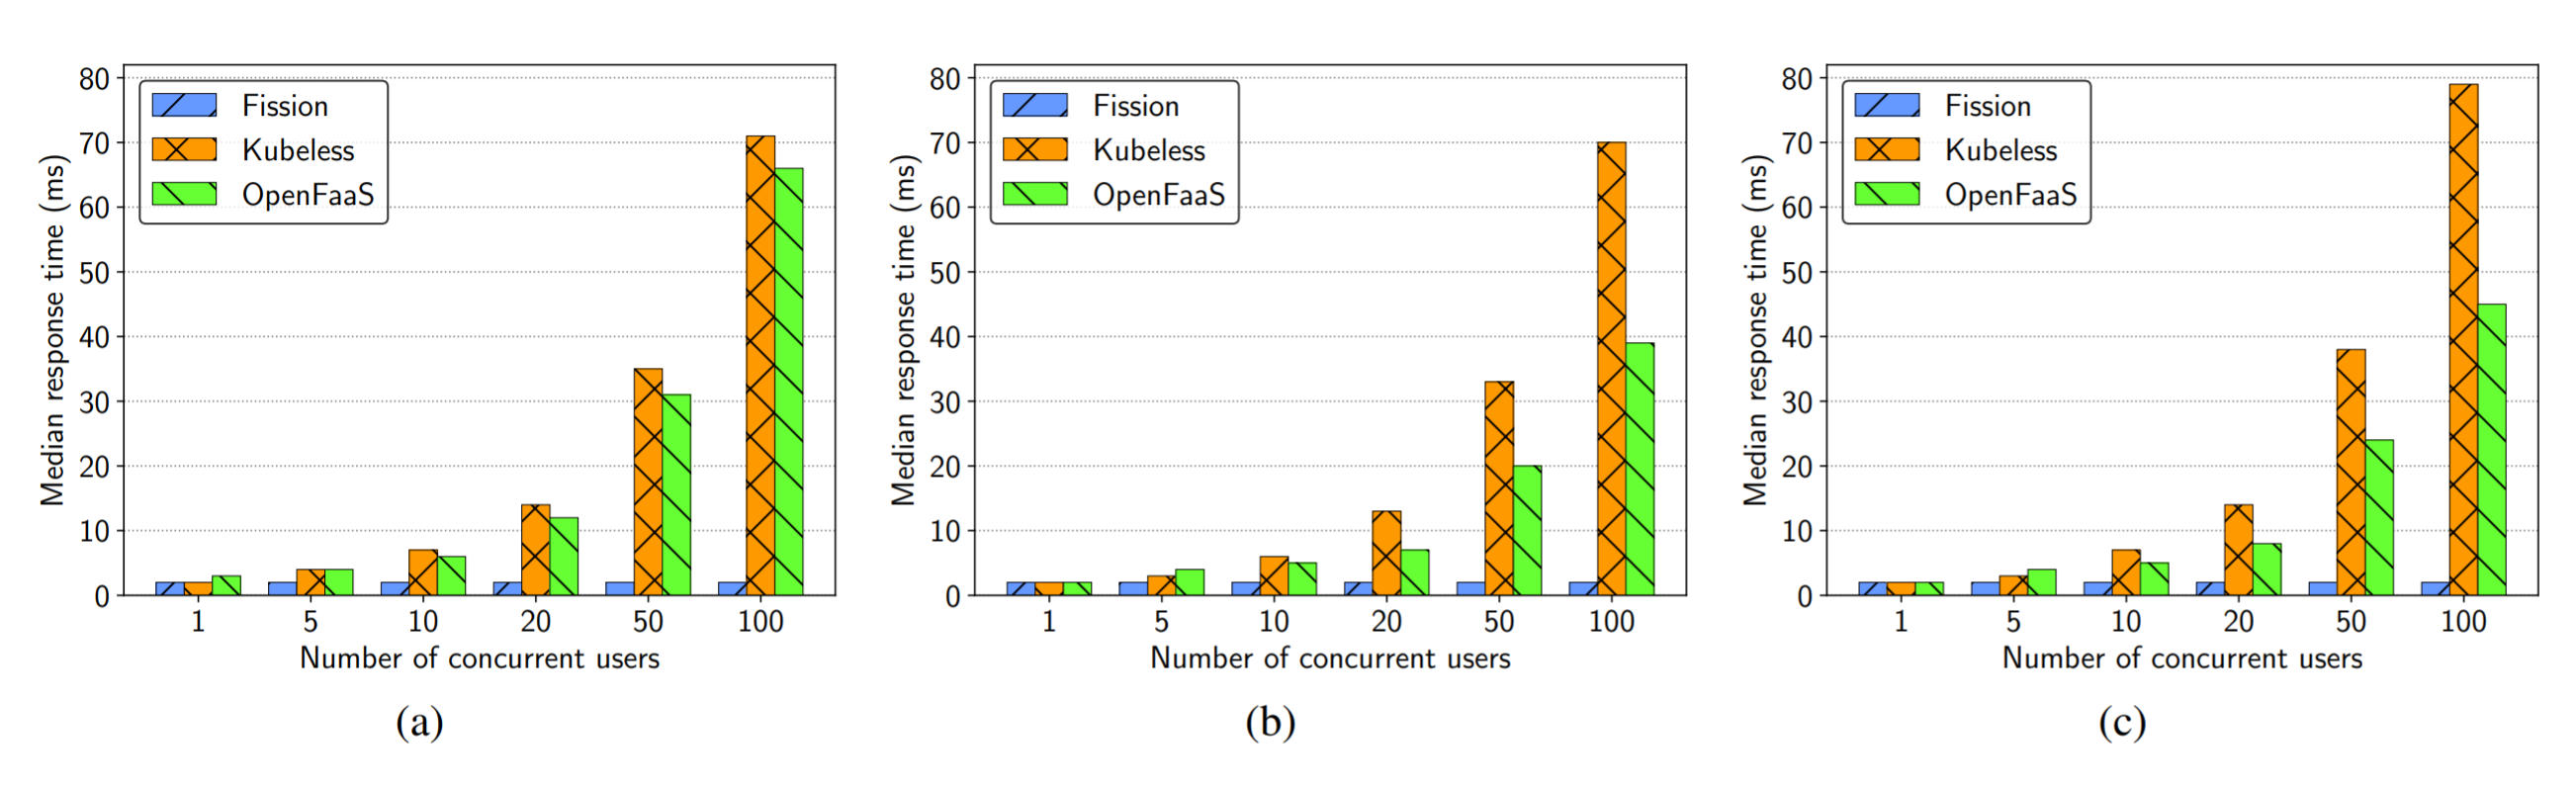
\includegraphics[width=1\textwidth]{opensource}
\end{figure}
\subsubsection{Proprietary Cloud-Providers}
Speaking of proprietary Function as a Service solutions, there are currently three market leaders with AWS, Azure and Google, respectively \cite{kumar2019serverless}. By offering a vast amount of tooling and services, it can be challenging to choose one of these three, even though their underlying model does not differ much. By all three providers, functions are billed on their number of incoming requests, the time a function runs to process a request, billed at a tenth of a second, and the memory allocated to a function. Due to the cloud, especially serverless, being such a volatile market, listing on pricing and memory size would presumably be obsolete in a few months and therefor this thesis is referencing to the provider's websites. Instead, performance evaluations, concurrency and runtime will be used as an indicator for choosing a platform.\\\\ Currently, on AWS, the maximum amount of time a single function will last is 15 minutes. After that time, the container the function is running in will be killed, no matter whether it has finished processing. On Azure Functions, 5 min are the maximum by default, which can be upgraded to 10 if needed. Google Cloud Functions comes last, with a standard execution time of one minute, which can be raised up to 9 minutes. Looking at the limits on concurrent instances, on AWS Lambda, the limit varies between 500 - 1000 depending on the region. Independently, the burst con  currency limit can reach a maximum of 1000-3000 concurrent instances. Those numbers only describe the initial limits, allowing to add each minute 500 additional instances. At this point, it is important to mention that these limits refer to an account, not a function. 1000 might sound a lot in this context, but depending on the number of functions, 1000 concurrent running functions can be reached quite fast \footnote{https://aws.amazon.com/lambda/}.\\\\ Regarding the execution time of AWS Lambda and Azure Functions, the platforms not only differ in the execution time of cold and warm starts but also when comparing two programming languages. As a compiler language, with its JVM, Java functions require more time to execute than an interpreted language like JavaScript. Tests have revealed, that there can be a significant gap receiving a result with a difference from 0.6 (JavaScript) and 1.7 (Java) seconds from cold to warm start on AWS and 9.8 (JavaScript) and 24.8 (Java) seconds on Azure \cite{manner2018cold}. Moreover, Manner et al. have detected that the cold start time of Java compared to JavaScript is on each memory size on AWS by a factor of two to three higher. Azure with a factor of 2.5 shows equal latencies in cold starts. Due to different memory allocation approaches, explicit configuration on AWS and dynamic allocation on Azure, the findings of latencies between the platform can not be compared to each other directly \cite{manner2018cold}.\\\\ Observed by other researchers as well, AWS appears to be very predictable in its memory size to performance ratio \cite{pawlik2019performance}. Even though the performance-memory ratio is stable, the maximum CPU-performance increase seems to be reached with 2048MB of memory. 3008MB exhibits only a slight improvement on AWS. IBM and Google experience similar ratios but not as stable. In terms of delay, on AWS it was incestigated that with more memory capacity the delay, when starting a new instance, decreases. On the other hand Googles start-up delays are generally constant and do not seem to be impacted by higher or lower memory sizes. On IBM tough, it seems that by requesting larger amounts of resources the consumption time to consume the instance or resources, increases \cite{pawlik2019performance}. Function throughput, which is an indicator of concurrent processing capacity, AWS reaches its maximum throughput most rapid, followed by IBM, Azure and Google, respectively. Whereas Google at the lower end increases throughput steadily, with a rise in calls, AWS stays sturdy at its maximum. IBM and Azure experience a small decrease over a long time.\\\\ Lastly looking at the runtime overhead of AWS, IBM, Google and Azure, on AWS it is almost evenly low regardless of a compiler or interpreter language. On Azure, C\# creates the least overhead, still being twice as much as AWS highest language runtime overhead, and Python the largest. On IBM the overhead is similarly high across the languages, and Google has the least overhead with Nodejs \cite{pawlik2019performance}.\\\\ 
\subsubsection{Orchestration and Concurrency}
 Another point to consider, when migrating parts of existing architecture to Function as a Service is orchestration. The orchestration solutions vary between different cloud and open-source providers. The respective orchestration tool decides upon performance when executing functions in parallel and upon runtime overheads. Moreover, pricing needs to be considered when configuring concurrency options across different providers. As mentioned before, depending on the memory size chosen, the performance can be increased, but pricing will increase as well. Whereas in small projects, concurrency and pricing might not be the main issue, in medium to large-sized projects, memory and pricing of the various providers should be taken into account.\\\\ As stated in section \textit{Benefits and Drawbacks} under \textit{statelessness} when chaining functions, passing state from the sending to the receiving function is key for intercommunication. With a higher speed of state-transfer, latencies are reduced. Only with a seamless interaction of functions, complex applications can be built on a larger scale. Looking at proprietary cloud providers, the two largest platforms, AWS Lambda and Azure Functions,  will be depicted and further investigated. On the side of open-source frameworks, OpenWhisk is taken into consideration.\\\\ Lopes et al. have investigated on the named frameworks in greater detail and detected significant differences in state transfer on both sequential and parallel orchestration \cite{lopez2018comparison}. For the tests conducted, all functions were executed on warm instances/ containers, to mitigate inaccuracies caused by varying cold-start times, see \cite{manner2018cold} and \cite{jackson2018investigation}. In terms of executing sequential functions, called sequential processing, IBM's Composer and ASF proved to be significantly faster compared to ADF. The overhead, describing the time that was not used to carry out any processing of business logic inside a function, was 1.1s for IBM Composer and 1.2s for AWS Step Functions with 40 functions connected in series. Azure Durable Functions, on the other hand, took 8s for the same 40 functions. In further implementations with [5, 10, 20, 40 and 80] it turned out, that IBM Composer only supports the orchestration of functions up to a number of 50 sequential functions. Anything beyond that limit has to be controlled by a third party orchestration tool \cite{lopez2018comparison}. ADF and ASF, on the other hand, can define workflows which can run for days and months.\\\\ The evaluation of the overhead for functions connected in parallel was carried out for ASF and ADF, solely. Starting with five functions and, as described above, scaling up to 80, the results showed a significant increase in overhead of Azure Functions. With a total of 80 functions, Azure Durable Functions with an average overhead of 32.1s had almost twice the volume of AWS Step Functions with an average overhead of 18.3s. The results also suggested that ASF is more reliable than ADF in predicting the overhead to be expected. Microsoft's overhead has not always grown exponentially like Amazon's, making it difficult to predict future behaviour.\\\\ When evaluating the suitability of parallel function execution, IBM's Composer dropped out of the test portfolio right from the start, since parallel function execution was not supported as of 2018 \cite{lopez2018comparison}. Meanwhile, 2020, IBM includes support for parallel execution of functions via Composer. Furthermore, IBM states that parallel execution is not restricted to a certain number of concurrent functions and can be configured as needed \footnote{https://github.com/apache/OpenWhisk-composer }. However, it is explicitly mentioned that the Composer theoretically has no limits, but OpenWhisk does. Exceeding OpenWhisk's limits of parallel execution will result in failures: \glqq[...] many concurrent invocations may hit OpenWhisk limits leading to failures: failure to execute a branch of a parallel composition or failure to complete the parallel composition [...]\grqq{} \footnote{https://github.com/apache/OpenWhisk-composer}. The current limitation of concurrent functions in OpenWhisk is placed at 100 functions per namespace.\\\\ Finally, the three orchestration solutions were examined concerning transferring application state. Due to the state limitation of ASF to 32KB that can be passed to the next function, the same size was chosen for the other two solutions as well. This time only five sequential functions were tested. In 2018 the official limit of IBM Cloud Functions was at 1MB, being raised upon 5MB by the time writing this thesis \footnote{https://cloud.ibm.com/docs/OpenWhisk?topic=cloud-functions-limits}. ADF enables state transfer up to 60KB. It was found that IBM Composer and AWS Step Functions had an overhead of 175.7ms and 168.0ms, respectively,  when executed without any additional payload. With payload, the overhead in ms for Composer was 298.4ms and 287.0ms for AWS Step Function, which represents an increase of 70\%, see figure ~\ref{fig: orchestration}. Azure Durable Functions stood out clearly in this test. With an overhead of 766.2ms without payload and 859.5ms with payload, the basic overhead is significantly higher than with the previous two but only increases by 12\% under load \cite{lopez2018comparison}.
\begin{figure}[H]
\caption{Overhead bei 5 sequentiellen Funktionen mit einem Payload von 32KB, nach \cite{lopez2018comparison}}
\label{fig:orchestration}
\centering
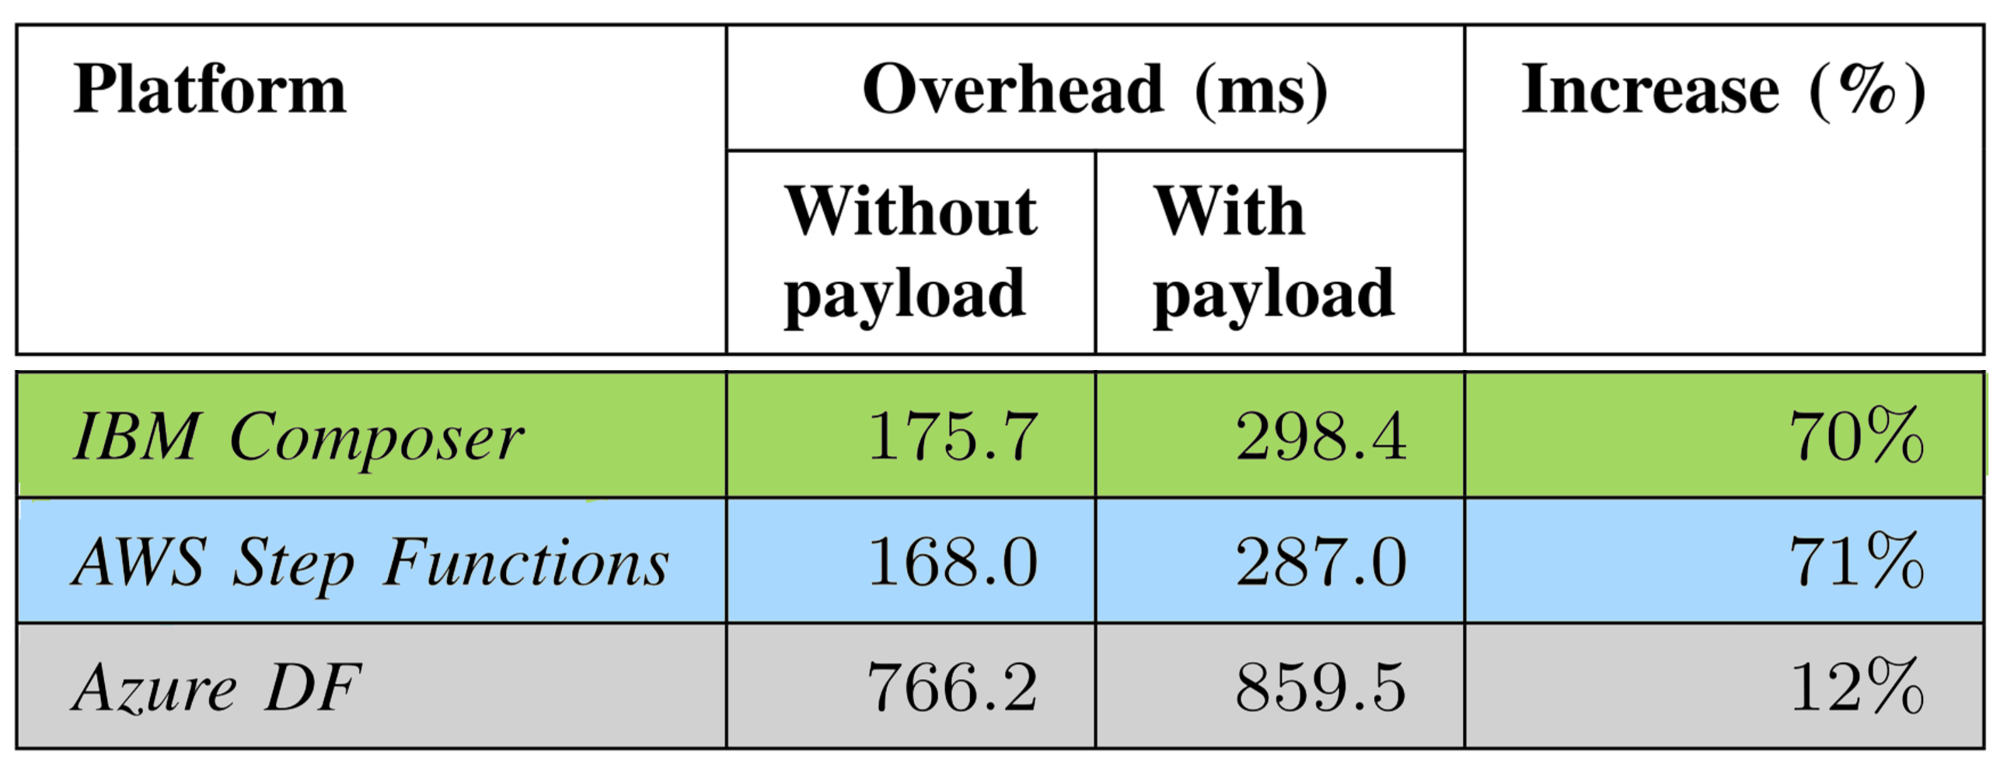
\includegraphics[width=0.7\textwidth]{Orchestration}
\end{figure} 
As shown by Lopez et al., AWS provides the most mature solution in terms of orchestration. Not only for sequential but also parallel execution AWS provides long-lived and short-lived function chaining. Also, the limitations on state transfer to 32KB enable AWS to provide clear information on pricing, compared with the other frameworks tested. When FaaS is mainly used for lightweight function chaining tasks, OpenWhisk in conjunction with IBM Composer is a suitable solution. With its limitation on chaining functions only up to 50 in number, OpenWhisk is slightly faster than AWS in that lower segment. For scheduling long-term running sequences, running for days or even month, OpenWhisk can not be recommended. If the focus is on the exchange of large application states between functions and more significant latency can be accepted, Azure is capable of such a use case. With a capacity of 60KB it its, by far, ahead of its competitors. Even sequences that run for an extended period can be configured. Moreover using async/await syntax with sequential function chaining and fan-out/fan-in\footnote{https://docs.microsoft.com/en-us/azure/azure-functions/durable/durable-functions-cloud-backup} for parallel execution, simplifies development over solutions from AWS and IBM \cite{lopez2018comparison}.
\subsection{Selecting a suitable service}
The service for starting the migration should manifest specific characteristics. As mentioned above, and in section two, \textit{benefits and drawbacks}, there are a view things that need to be taken into account. Due to Javas CPU-intense runtime and the time for loading potentially large amounts of libraries, the language is likely to raise the time of cold starts, eventually resulting in higher latencies \cite{bardsley2018serverless}. Also, the object-oriented model of Java must be restructured to meet the requirements of the original functional programming style of FaaS. Concepts embraced by Java, such as getters, setters, empty methods, constructors, and singletons, need to be considered when mapping an object-oriented programming language to decoupled functional units.\\\\ Considering these additional steps of migrating a service, written in an OOP language \cite{leitner2019mixed}, it might be more rational to start with a service written in a functional programming language. The development team has to decide on the issue of refactoring in favour of rewriting. When the goal is to maintain consistency in language, accross the entire platform, the former decision is in favour. Otherwise, converting the service into a functional language, by rewriting it, could be another option. In the latter case, JavaScript, PHP, and Python, primarily being functional functional, are suitable candidates for conversion.\\\\ Furthermore, the majority of practitioners use functional programming languages over OOP languages \cite{leitner2019mixed}, increasing the likelihood of finding solutions to problems on the internet. In contrast to legacy applications and the majority of PaaS and IaaS architectures, the service that is about to be converted should not experience permanent high traffic. \textcolor{blue}{Besides that, looking at the existing microservice architecture and identifying services that spend most of their time in IDLE, can be considered for migration.} \textcolor{green}{Weiter darauf eingehen. Und use-cases an dieser stelle noch einbauen}
\subsection{Effects on development}
During development, teams are working according to certain process models, trying to improve their efficiency. Therfore different tools and frameworks are used to enhance productivity and improve working velocity. Some are utilized in order to maintain the platfrom, to not lose track of its present state, others apply on the actual coding/ service-development process. Nevertheless with changes in technical concepts new operational and organizational cahnges evolve. In the following several effects of Function as a Service on the existing structures will be investigated on. % \subsection{Effects on teams, development and tooling}
\subsubsection{Impact on Teams}
When a microservice architecture is prevalent, FaaS can be adopted with fewer changes than a monolithic architecture \cite{fox2017status}. With a microservice architecture, concepts like agile development, continuous delivery and continuous integration, as well as a different mindset amongst the development team, are probably more common. Nevertheless, FaaS goes a step further, then developing microservice with PaaS does, which suggests the assumption that the PaaS-adapted development structure will change.\\\\ Starting with agile development and \glqq DevOps\grqq{}, Function as a Service forces companies and teams to adopt an agile mindset and agile techniques \cite{benlian2018transformative}. The necessity of iterative cycles is accounted for by the concepts great modularity compared to microservices. Persuing procedures form older waterfall driven projects are still prevalent, the implications of the sequential process model would not satisfy the needs of Serverless, respectively, FaaS. With a significant reduce in lead time development, long periods of requirement engineering will hinder the effectiveness of FaaS. Teams that already incorporated agile process frameworks, such as scrum, will have an advantage over those still remaining to acquire experience. Serverless development will enhance the importance of continuous delivery and continuous integration. Integrating procedures like unit testing and integration testing, to diminish time to market to a minimum, need to be further investigated. Depending on the size and complexity, which should be kept to a minimum as well, the chances are that FaaS will be considerably faster than the current microservice development. To prepare for integration, slow processes have to be identified and eiter speeded up or thier effects mitigated. This way bottlenecks will be eliminated.\\\\ Furthermore, the size of the teams, to be more accurate, the number of developers working on a function, should experience a decrease. Whereas now two to four developers are working on a microservice, this number likely gets reduced to only one developer for each function. With separation of concerns and further decoupeling functionalities of a service, FaaS naturally decreases complexity, at least on the code level. Also, reducing complexity and focussing on a specific functionality can help to optimize each function further. By doing so, besides the reduction in startup latency, with the shorter execution time, the platform will charge less \cite{shafiei2020serverless}.\\\\ 
\subsubsection{Version Control System}
 However, when maintaining a microservice infrastructure, each service and each version is likely to have a separate repository. With Function as a Service, this approach will be challenged regarding the number of functions that make up the application or service. Having a repository for each function, the odds are in favour of experiencing an overhead in version control and keeping track on the application landscape. Hence teams pursuing this approach are facing duplication in their code base, because the existing functions, can not be gathered with little effort \cite{racicot2019quality}. This complexity and duplication seem to be the cause of why many users follow a mono-repository approach over having many small repositories \cite{brousse2019issue}.\\\\ With that said, FaaS seems to be conflicting with itself to some extent. Although its modularity suits the poly-repository approach quite well, ther is accompanying complexity, while an application keeps growing. Not having a clear overview of the codebase and especially a potentially vast amount of functions redundancy is likely to increase. The consequence of that is inefficiency while maintaining and expanding the application landscape. This is in a sort analogous with the scripting practice in larger software projects. If a quick fix for incompatible components is needed, a script is often used to cope with the issue. The results are myrads of scripts, that are had to maintain, because the next problem is likely to be fixed by another script. In parctice, the scripts of are not in one place, probably even stored in the repository of the service itslef. Providing they are strongly context bound, this is not a big issue, but many time they are of a far more general nature. Resulting in a lack of reusability, redundancys are faced and efficiency is reduced [\textit{internal source}].\\\\ As a suggestion, there should be a mono-repository-approach for each (Scrum)-team and a ploy-repo approach for each division. Both would coexist with the present VCS of the microservice-architecture. This way, redundancy of code in a team is kept very low, by simultaneously having a manageable amount of repositories across a division of a company. With this approach, complexity can not be eliminated, but at least mitigated to a certain degree. Moreover, having seperated repositories for different teams will simplify the use of many accounts for development and production, as discussed in a later section.\\\\ 
\subsubsection{Programming Language}
 Another issue that can emerge during the process of development is affected by the programming language used. Looking at Java, which mainly is an object-oriented programming language, even tough concepts such as Lambdas, added in version eight, the question of refactoring arises. However, besides these Lambda expressions, the core of a Java application is OOP-based. Migrating microservies that are Java-based to FaaS, it is necessary to map Java classes to functional units that can be deployed onto the serverless platform. Moreover, concepts like empty methods, getters, setters, constructors and singletons have to be taken into account \cite{spillner2017Java}. Looking further, the absence of conventions outside the actual code, like the usual presence of a \textit{src}-folder, have to be investigated. During the process of transformation, the Java-based services need to be split up into bounded contexts allowing the business logic to be seperated. With regard to the effects of many dependencies, a reduction of mutual dependencies has to be made to decreasing startup latencies. Two functions should not load the same dependencies if not necessary. This way, startup latencies will be kept to a minimum. Spillner et. al suggested an approach to automatically transform Java code to AWS-Lambda functions, consisting of six steps.
\begin{itemize}
  \item[1.] Conducting a static code analysis based on the service code in the VCS.
  \item[2.] Decomposing the code into context-bound parts.
  \item[3.] Translating the split code into functional units which are uploaded to a target repository. 
  \item[4.] Compiling the code and inspect issues and failures and upload the code to the binary repository. 
  \item[5.] Deploy the data form the binary repository to AWS
  \item[6.] Test and verify the code.
\end{itemize}
Even though the last two steps are Lambda specific, the former ones provide a generic starting point. Unfortunately, this concept, especially in conjunction with automation, is as stated by \cite{spillner2017Java} only applicable for simple Java applications. Moreover, migrating from an object-oriented approach, respectively Java, state changes in classes and objects need to be treated separately. In a functional unit, keywords such as \textit{this}, referencing itself in a Java-class, are not applicable. To address this issue, the self-reference, as suggested by Wright et al. \cite{wright1998compiling}, should be provided with the method signature that is passed to a function. This way, the same underlying object structure can be equally invoked with every new instance of a function being started. Operations on the container do not interfere with objects in other containers, and saving the state in external databases will not cause redundancy between the different objects \cite{spillner2017Java}.\\\\ 
\subsubsection{Tooling and Multi-Cloud}
Literature is currently facing a lack of tooling, in terms of the variety and maturity provided by present sloutions \cite{Yussupov2019_SystematicMappingStudyFaaS}, \cite{leitner2019mixed}. With a share of around 80\% \cite{leitner2019mixed} of practitioners using the Serverless\footnote{https://serverless.com/} framework, this tool is the most frequently used in the market. Besides the Serverless Framework, Terraform\footnote{https://www.terraform.io/} and CloudFormation\footnote{https://aws.amazon.com/cloudformation/} are mentioned as well, but their appearance is far less. Especially in conjunction with the CI/CD pipeline, the use of tooling can play an important role. By using one of the tools mentioned above, the deployment is configured withing those tools, providing an abstraction layer between the contemporary architecture and the provider's platform.Thereby these tools enable hybrid architectures across multiple cloud providers. Terraform and the Serverless Framework both manage resource configuration and therefore need to be connected with the providers. The connection will be established depositing authentication data for all cloud solutions to be managed on the framework. By striving to gain independence and reduce the effect of vendor lock-in [see \textit{benefits and drawbacks}], these frameworks are supporting that process. Especially the Serverless Framework, thanks to its vast amount of plugins, provides, e.g. an offline simulation of AWS Lambda and the AWS Gateway \cite{lin2018tracking}.\\\\ Within this conjunction, additional operational tasks should not remain unmentioned. Even though Serverless, Terraform, and CloudFormation provide the opportunity to register many accounts from all kinds of serverless providers, including AWS, Azure, IBM and more, they face an initial load in configuration. Another issue that needs to be addressed is that new features offered by a platform will not be adjusted to third parties, which engenders latency time until the third party might provide the feature. Thus, these IaC frameworks do not come for free\footnote{https://serverless.com/pricing/}. They can be used for free to a certain extent, but when it comes to more advanced tasks, they will charge the user. Finally, they do as well represent some vendor lock-in.\\\\ Depending on the purpose of multi-cloud solutions, there might be higher costs than using just one provider. If functions form one provider need to access another's providers function, its functions will be affected by cold starts. Moreover, the physical distance between the two data centres will affect latencies. If the primary purpose of deploying an application to different cloud providers is to have redundant systems in case one fails, the cost will not be affected too much. Still, additional operational tasks are required to guarantee a stable backup. Testing needs to be done not only on one but on all cloud providers, the application is mirrored to, which will cause additional costs besides the operational overhead of monitoring and testing.\\\\ Regarding the deployment pipeline, in practice, many tasks are handled via scripts, as mentioned before. Introducing serverless, special tooling for deploying a function to the desired platform is necessary and needs to be included in the existing pipeline. If not using one of the IaC frameworks mentioned above, the providers specific CLI has to be integrated, in the case of AWS Lambda CloudFormation. Integration can vary depending on the provider but is inevitable, according to practitioners \cite{ivanov2018implementation}.
\subsection{Effects on Testing}
There are several ways to test a serverless application. A distinction is made between local unit-testing, canary releases, as well as A/B testing and integration testing. While OpenWhisk was the first framework offering local unit testing, the other providers have adopted this as well. Looking at AWS, Amazon provides with their open-source Serverless Application Model (SAM)\footnote{$https://aws.amazon.com/de/serverless/sam/?nc1=h_ls$} the possibility to build, test and debug the application locally. On Azure, Microsoft provides the so-called \textit{Function Core Tools} as integration for running functions locally\footnote{https://docs.microsoft.com/en-us/azure/azure-functions/functions-develop-local}. Even though the underlying business logic can be tested locally, there is no guarantee that the code will work the same when the function is deployed into the actual ecosystem. A reason for that is the interaction with triggers, events, databases, functions and other services which, again, can not be simulated accordingly in a local environment. In contrast to that, hosting an application on-premise or via IaaS or PaaS, it often is possible to not only unit-test locally but also simulate integration testing locally. Due to being in charge of the platform, there are often local copies of databases or message queues which are quite similar or identical to those running in production. Not only are there copies but real databases that can be accest locally far more easy, due to being in charge of the \glqq database-service\grqq{}\\\\ Moreover, it is hard to provide all configurations made on the different services locally. Key figures, such as the execution time of a function, the speed of loading all dependencies and potential latencies due to cold starts will be different on the cloud platform. Also, the unawareness on which type of server the function will be started makes predictions on performance difficult \cite{racicot2019quality}. Due to the complexity being abstracted to the cloud vendor, the user has no further control over these services, ececpt of what the platform allows them to do. This restriction is not affected when performing unit tests, which is very easy, based on the small code base of the functions. With all these implications, it is inevitable to test the service on the provider's platform to get reliable results on compatibility and performance, even though tested locally.\\\\ When testing on the platform, there are several possibilities that can be chosen form. Starting with canary releases, considering the size of serverless functions, changing solely specific behaviour becomes far more feasible. After a new version is deployed, changes can be made to the API-Gateway of the serverless platform, in order to redirect a defined group of users. These cloud then test only a new version of a function or the entire application. Without being charged for code stored on the platform, only for code being run, it is possible to mirror the entire application to another account, without experiencing an increase in pricing. On that account, the new feature can be tested. Regarding the operational overhead of the mirroring process, mirroring appears to be more comparative on major changes to the application and or a function. For patches, solving defects, or minor changes, adding new features to an application, not affecting is API, the effort of mirroring might not be necessary. Using AWS, Azure or Google, canary releases can be scheduled via the CLI. On AWS in particular, canary releases can be achieved either via \textit{aws-lambda-deploy} or AWS Step Functions. Although the opportunity of canary releases and A/B testing theoretically exist, it is not very often used by operators \cite{leitner2019mixed}. One reason cloud be the operational overhead, another the implications on performance, when not having a separate development and production account. Especially load tests are likely to affect performance on an account. In case only one account is used for testing and production, latencies can have a noticeable effect on the application, affecting end consumers. Therefore, it is advisable to have at least two different types of accounts — one for production and one for testing purposes. Despite the additional overhead, load tests can be done safely without any impact on the actual application \cite{leitner2019mixed}.
\subsection{Implications on monitoring}
Debugging and monitoring are crucial parts of any application. They ensure that the application is stable. The two metrics are indispensable in determining the health of an application during testing and later on in production. After going through the different testing environments, DEV, INT, UAT right up to PRD, the data gathered can be used as a baseline of the normal behaviour of a service. Whenever running out of memory or failing to provide a new instance of a service, the monitoring solution will, in a perfect world, alert the operator before issues in production cause severe damage. Whereas the team has full control over their servers when using a PaaS or IaaS solutions, with a container environment like Kubernetes on top, it is quite different when switching to FaaS.
\begin{figure}[H]
\caption{Monitoring cloud functions, by \cite{manner2019troubleshooting}}
\label{fig:manner}
\centering
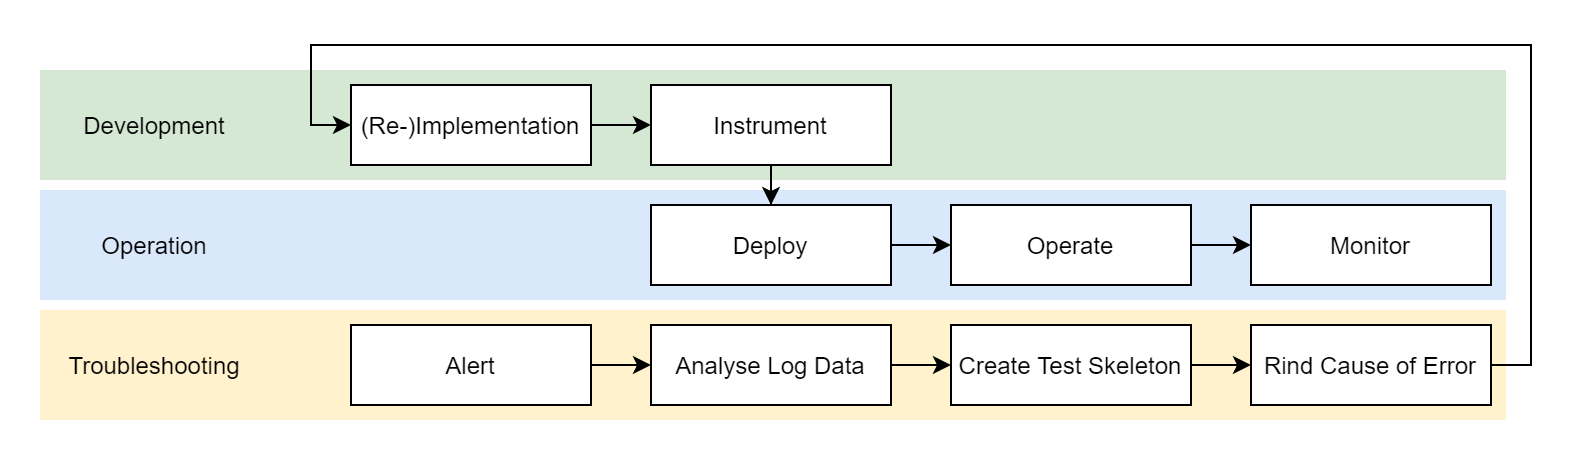
\includegraphics[width=1\textwidth]{monitoring}
\end{figure}
According to several papers [\cite{roberts2017serverless}, \cite{baldini2017serverless}], the field of serverless, mainly Functions as a Service, exhibits a lack of monitoring, logging and debugging solutions \cite{kritikos2018review}. Facing a lack of custom metrics, the operator solely relies on logging additional information needed, that are not provided by the platforms monitoring service. Not having access to the platforms infrastructure, bound to the autonomy of the cloud provider for provisioning his platform. Enabling precise debugging on the environment would, as stated by \cite{manner2019troubleshooting}, take away the provider's control, to free capacity when not needed and scale functions as efficient as possible. Due to not having any control over the platform, it is crucial to monitor the functions constantly. In order to address this issue, Manner et al. provide a monitoring and debugging approach. Because of its comprehensiveness, it will be recommended to be used for setting up a monitoring and debugging solution for cloud vendor platforms. For convenience only, figure ~\ref{fig:manner} shows the concept proposed by Manner et al. in a slightly modified way. The concept is split into three segments, namely development, operation and troubleshooting.\\\\ In the development-phase, the function should be implemented with three parameters that are going to be logged to an external database or monitoring service. These parameters are the input, the context and the output of the function which is being called. The limitation to three parameters is chosen, to not have too many repercussions on the execution time of the function. At the same time, the functions are providing enough data to reproduce failures when they occur \cite{manner2019troubleshooting}. After the functions have been tested on a development account, they will be forwarded to the production account. As a result of this, a clear distinction between the production and the development account is not necessary since they are identical. \\ In the second phase, the operational phase, the developer has to make use of monitoring services, which collect the data logged from each function. The received logging data will be further processed to determine a corridor for the execution times of a function. Whenever a function falls underneath a predefined execution time, an event will be triggered, which informs the operations team. In DevOps there is no seperation between developers and operatior. The developers are, as well as the operators, in charge of the product they have built, according to the concept: \glqq You build it, you run it!\grqq{}.\\ With an alert beeing send, the troubleshooting-phase is launched. In order to create a test skeleton consisting of the three logged parameters, all functions failed or exceeding the corridor are filtered to retrieve their logging-data. Afterwards, the placeholders of the skeleton are replaced with the actual data to find the cause of the error \cite{manner2019troubleshooting}. This process will ideally be combined with the development account, not to affect the performance of the production account. At last, it is essential to log the data asynchronously before the function returns a response. After returning a response, the container will be discarded immediately stopping any processing.\\\\ Regarding open-source frameworks, it is crucial to be aware of the modularity which comes along with Function as a Service. When monitoring an environment, logging data from services and complementary parts will be collected. The data collected has to be stored within a database, being able to run aggregation, sorting and other types of evaluation metrics upon. Implementing an open-source FaaS framework into existing infrastructure, function monitoring can be included in the present monitoring solution. Being in charge of the infrastructure, metrics can be collected on a far deeper scale, e.g. the container runtime itself and as well as from the underlying OS. In case the former landscape consists of several more extensive services, potential bottlenecks need to be determined and have to be eliminated. The bottlenecks could occur in the form of connection pools to databases and need to be adjusted. With potentially many functions, that again have many instances; the connection pool has to scale dynamically. Another solution is a central message queue; all functions can provide their logging data to. As the message queue usually is faster than the database, it will collect the asynchronously logged data and forward it to the database.
\subsection{Results}
With respect to the present microserive architecture, migrating to FaaS is going to effect many parts of development and operatins. Due to the prevailent modularity though, changes on development are rather minor changes, provided an agile process model and agile developemnt is practiced. Regarding operations, major changes can be seen, affecting the application landscape. Figure ~\ref{fig:devopsModified} depicts the observed changes of migrating to FaaS compared to the present landscape, first presented in section \textit{Describing the existing architecture}. \\\\ 
\begin{figure}[H]
  \caption{Modified DevOps pipeline}
  \label{fig:devopsModified}
  \centering
  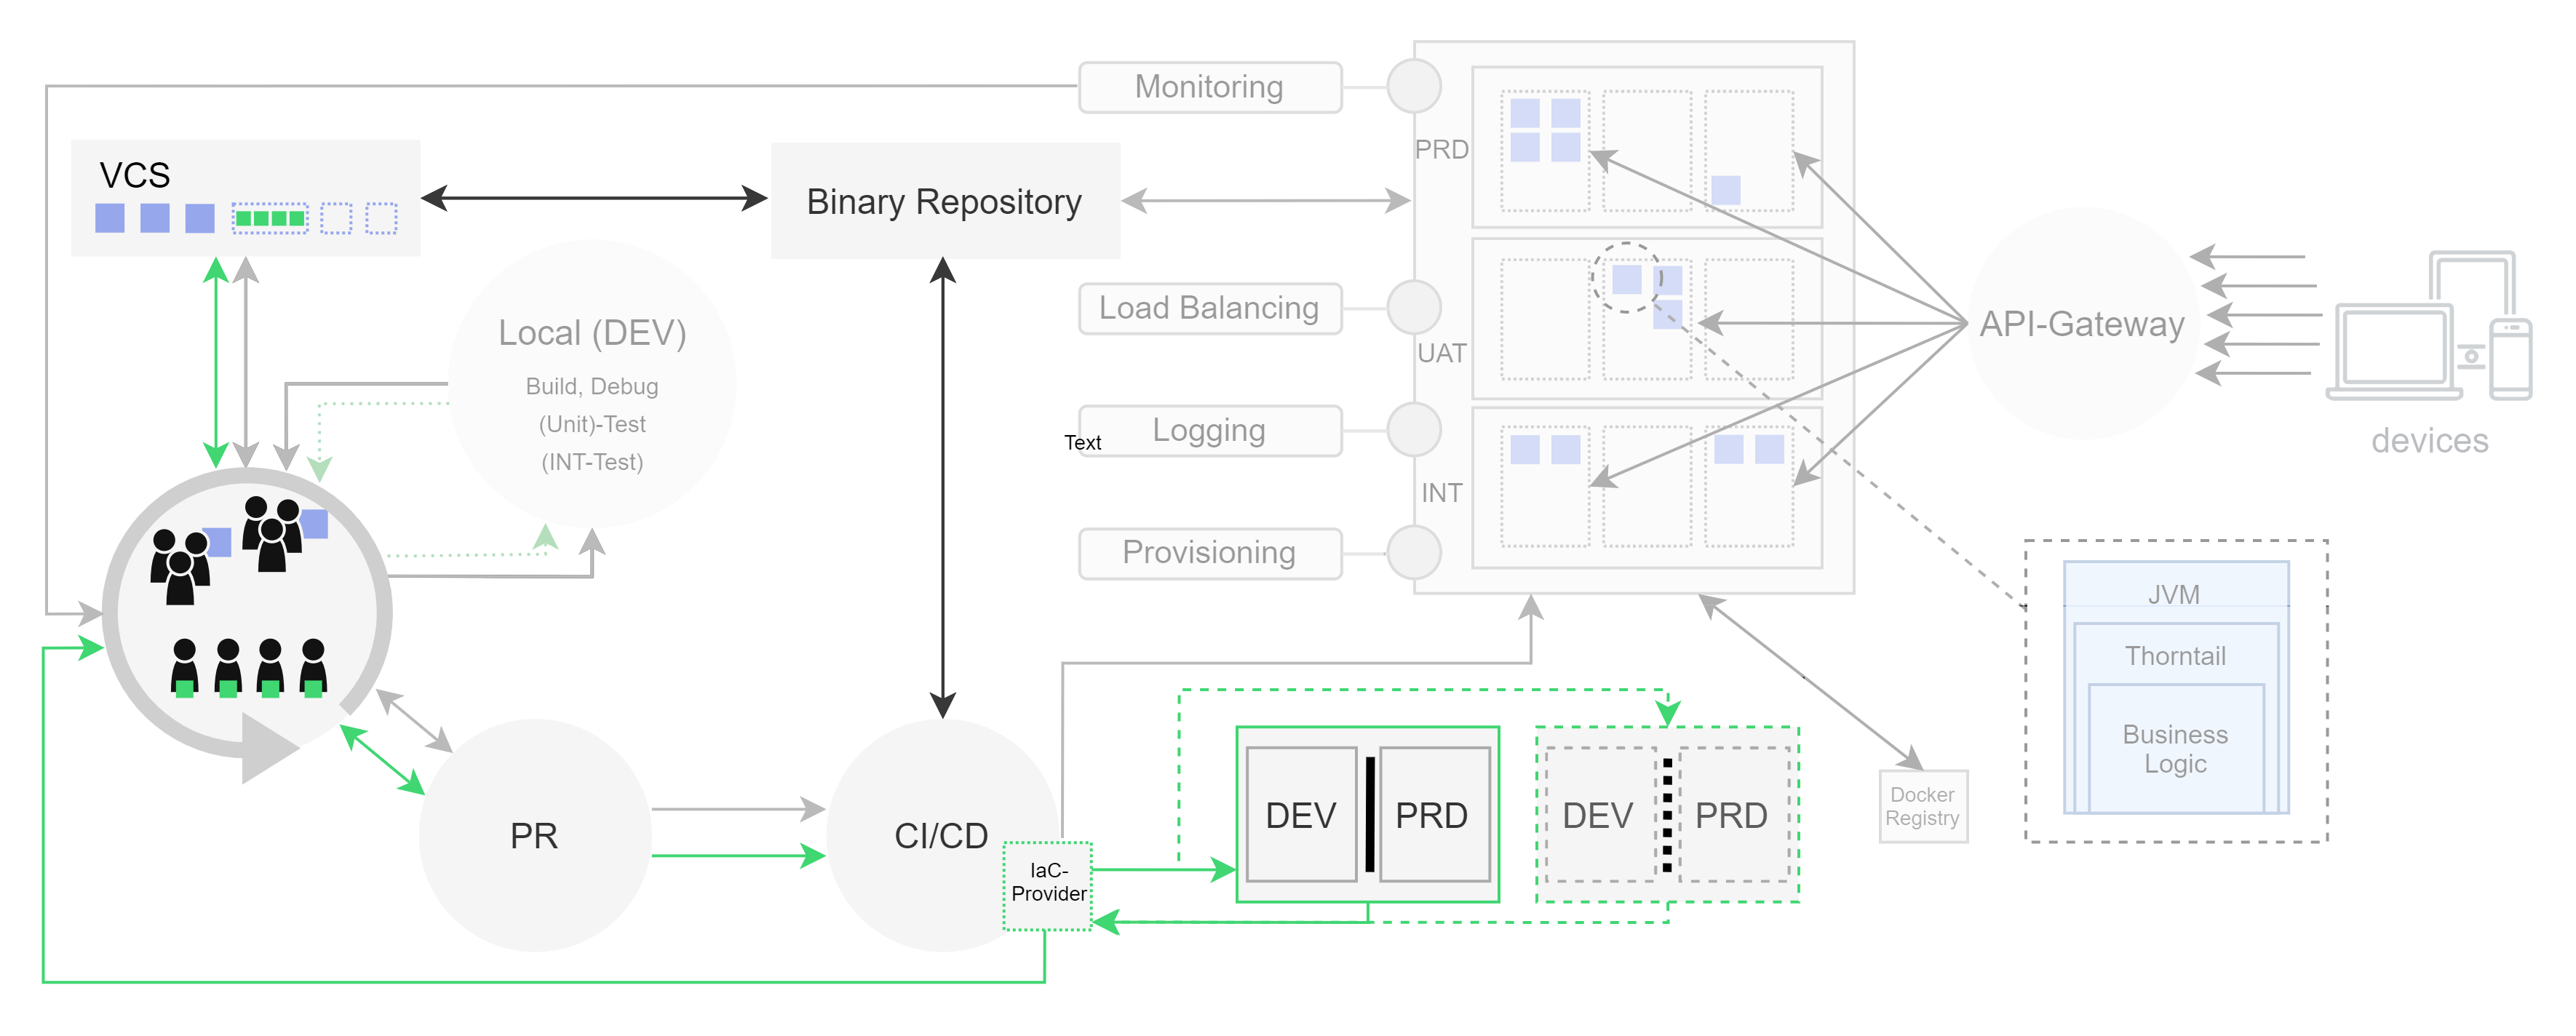
\includegraphics[width=1\textwidth]{devopsModified}
\end{figure}
\newpage
\section{Anwendung des Leitfadens}
\subsection{Auswertung der Ergebnisse}
%Before starting with the prctical part of migration, the soundess of the migration purpose needs to be examined.  With migrating to FaaS many parts of the existing microservice architecture are effected and have to be adjusted. With regard to the present microservice architecture migrating parts of the Hypothesis 1: Computational performance of a cloud function is proportional to function size.This is true for AWS Lambda and Google Cloud Functions, with the exception of about 5\% cases when Google function runs faster than expected.This is not true for IBM and Azure since the performance does not depend on the function size.Hypothesis 2: Network performance (throughput) of a cloud function is proportional to function size.This is confirmed for AWS and Google, with the same restriction as Hypothesis 1. We have not measured transfers for IBM and Azure, so this stillneeds to be verified.Hypothesis 3: Overheads do not depend on cloud function size and are consistent for each provider.This hypothesis was generally confirmed for all the providers.Hypothesis 4: Application server instances are reused between calls and are recycled at regular intervals.This was nicely demonstrated by our experiments, and we also observed that the instance lifetime differs between providers.Hypothesis 5: Functions are executed on heterogeneous hardware.While we were able to get results only for two of four providers, we can clearly see that the hardware that runs FaaS infrastructure isheterogeneous.We have to note that, while our hypotheses are generally confirmed, the most interesting observations are those when we see some exceptionsor deviations from the general patterns. The specific resource allocation policies as these of Google or different variances of the results have to betaken into account when making decisions about choosing the provider and the function size. Moreover, the price/performance analysis needs to becarefully performed to avoid unnecessary costs




% INT UAT und Prod aus gutem Gund, aufgrundvon  e2e sowie lpts der verschiedenen Services. In finanysektor vor allem bei last tests ... lack of focus on  large scale enterprise applications \cite{kumar2019serverless}.
%Adopting serverless requires a different mental model, where systems are primarily constructed by composing pre-existing services, with FaaS often acting as the “glue” that brings these services together. FaaSofferstechnicalandbusiness-relatedadvantages, but managing and predicting deployment costs is difficult for larger applications. Further, tooling availability and maturity, especially related to testing and deployment, remains a barrier to entry. Finally, limited support for function sharing and the absence of a service ecosystem is seen as a challenge.  \cite{leitner2019mixed}, 
% With FaaS, memory problems are less dangerous. Any OBject affecting heap or stack, wont matter to the platform, due to the functions being suspeded after returning a resonse or exceeting the timelimit of the platfrom. 







 
%  Factors that influence the modifiability are the amount of duplicated code, the complexity of the code units and the coupling between the modules \cite{racicot2019quality}. 



% Configuring memory for thorntail JVM ... from the two GB a pod can provide

% Another issue that arises are scrity concerns. 
\subsubsection{Beurteilung der Kollaborationsauswirkungen}
\subsubsection{Beurteilung der Stabilität}
\subsubsection{Beurteilung der Skalierbarkeit} 
\subsubsection{Beurteilung des Monitorings}
\subsubsection{Beurteilung der Testmöglichkeiten} 
\subsection{Korrektur und Anpassungen}
\section{Abschließende Betrachtung}
\subsection{Absehbare Entwicklungen}
% \cite{al2019systematic} Serverless  immer mehr bekanntheit und mehr Papers etc. ... Später market für funktionen die optimiert sind etc. \cite{shafiei2020serverless}\\
% Real time communication tool  \cite{shafiei2020serverless} \\
% Real time tracking gps  \cite{shafiei2020serverless} da beide nicht auf dem Application state benötigen/ beruhen  \cite{shafiei2020serverless} \\
% \cite{hellerstein2018serverless}
\subsection{Zusammenfassung}
\subsection{Weiterführende Forschung}
% Serverless Computing: A Survey of Opportunities, Challenges and Applications store for functions
% \cite{shahrad2019architectural}
\newpage
\printbibliography%[title={Literaturverzeichnis}]
\end{document}